% adopt PLoS genetics environment settings
\documentclass[10pt,letterpaper]{article}

% Load to combine multiple standalone tex files into Supplemental Material
\usepackage{standalone}

% Template for PLoS
% Version 3.2 March 2016

% General commands for the entire paper
%
% Use Unicode characters when possible
\usepackage[utf8x]{inputenc}
% amsmath package, useful for mathematical formulas
\usepackage{amsmath}
%\usepackage{natbib}
% amssymb package, useful for mathematical symbols
\usepackage{amssymb}
\usepackage{booktabs}
\usepackage{xspace}
\usepackage{hyperref}
% graphicx package, useful for including eps and pdf graphics
% include graphics with the command \includegraphics
\usepackage{graphicx}

% Use adjustwidth environment to exceed column width (see example table in text)
\usepackage{changepage}

% textcomp package and marvosym package for additional characters
\usepackage{textcomp,marvosym}

% fixltx2e package for \textsubscript
\usepackage{fixltx2e}

% cite package, to clean up citations in the main text. Do not remove.
\usepackage{cite}
\usepackage{caption}
\usepackage{subcaption}
\usepackage{rotating}

\usepackage{color}

% Use doublespacing - comment out for single spacing
%\usepackage{setspace}
%\doublespacing

% Text layout
\topmargin 0.0cm
\oddsidemargin 0.5cm
\evensidemargin 0.5cm
\textwidth 16cm
\textheight 21cm

\setlength{\parskip}{1em}

% Bold the 'Figure #' in the caption and separate it with a period
% Captions will be left justified
\usepackage[labelfont=bf,labelsep=period,justification=raggedright]{caption}

% Use the PLoS provided bibtex style
\bibliographystyle{/Users/stephens/Dropbox/Documents/stylefiles/plos2009}

% Remove brackets from numbering in List of References
\makeatletter
\renewcommand{\@biblabel}[1]{\quad#1.}
\makeatother

% Use nameref to cite supporting information files (see Supporting Information section for more info)
\usepackage{nameref,hyperref}

% line numbers
\usepackage[right]{lineno}

% ligatures disabled
\usepackage{microtype}
\DisableLigatures[f]{encoding = *, family = * }

% Leave date blank
\date{}

\pagestyle{myheadings}
%% ** EDIT HERE **
\usepackage{enumerate}
\usepackage{multirow}
\usepackage{url}
\usepackage{xr} %for cross-referencing
%% ** EDIT HERE **
%% PLEASE INCLUDE ALL MACROS BELOW
\newtheorem{algorithm}{Algorithm}
\newtheorem{proposition}{Proposition}
\newtheorem{restateproposition}{Proposition}
\newtheorem{lemma}{Lemma}
\newtheorem{corollary}{Corollary}
\newtheorem{result}{Result}
\newtheorem{note}{Note}
\newtheorem{definition}{Definition}

\def\KL{\text{KL}}


% Text layout
\raggedright
\setlength{\parindent}{0.5cm}
\textwidth 5.25in
\textheight 8.75in

% Bold the 'Figure #' in the caption and separate it from the title/caption with a period
% Captions will be left justified
\usepackage[aboveskip=1pt,labelfont=bf,labelsep=period,justification=raggedright,singlelinecheck=off]{caption}
\renewcommand{\figurename}{Fig}

%------ bibliography
% Use the PLoS provided BiBTeX style
\bibliographystyle{plos2015}
% Remove brackets from numbering in List of References
\makeatletter
\renewcommand{\@biblabel}[1]{\quad#1.}
\makeatother


% Header and Footer with logo
\usepackage{lastpage,fancyhdr,graphicx}
\usepackage{epstopdf}
\pagestyle{myheadings}
\pagestyle{fancy}
\fancyhf{}
\setlength{\headheight}{27.023pt}
\lhead{\includegraphics[width=2.0in]{PLOS-submission.eps}}
\rfoot{\thepage/\pageref{LastPage}}
\renewcommand{\footrule}{\hrule height 2pt \vspace{2mm}}
\fancyheadoffset[L]{2.25in}
\fancyfootoffset[L]{2.25in}
\lfoot{\sf PLOS}

%% Include all macros below

\newcommand{\lorem}{{\bf LOREM}}
\newcommand{\ipsum}{{\bf IPSUM}}

%% END MACROS SECTION

%% Author's settings
\def\KL{\text{KL}}


% Text layout specific to Supplemental Materials
\topmargin 0.0cm
\oddsidemargin 0.5cm
\evensidemargin 0.5cm
\textwidth 16cm
\textheight 21cm

\setlength{\parskip}{1em}

\begin{document}

\section{Supplementary figures}
% adopt PLoS genetics environment settings
\documentclass[10pt,letterpaper]{article}
\usepackage[top=0.85in,left=2.75in,footskip=0.75in]{geometry}

% Template for PLoS
% Version 3.2 March 2016

% General commands for the entire paper
%
% Use Unicode characters when possible
\usepackage[utf8x]{inputenc}
% amsmath package, useful for mathematical formulas
\usepackage{amsmath}
%\usepackage{natbib}
% amssymb package, useful for mathematical symbols
\usepackage{amssymb}
\usepackage{booktabs}
\usepackage{xspace}
\usepackage{hyperref}
% graphicx package, useful for including eps and pdf graphics
% include graphics with the command \includegraphics
\usepackage{graphicx}

% Use adjustwidth environment to exceed column width (see example table in text)
\usepackage{changepage}

% textcomp package and marvosym package for additional characters
\usepackage{textcomp,marvosym}

% fixltx2e package for \textsubscript
\usepackage{fixltx2e}

% cite package, to clean up citations in the main text. Do not remove.
\usepackage{cite}
\usepackage{caption}
\usepackage{subcaption}
\usepackage{rotating}

\usepackage{color}

% Use doublespacing - comment out for single spacing
%\usepackage{setspace}
%\doublespacing

% Text layout
\topmargin 0.0cm
\oddsidemargin 0.5cm
\evensidemargin 0.5cm
\textwidth 16cm
\textheight 21cm

\setlength{\parskip}{1em}

% Bold the 'Figure #' in the caption and separate it with a period
% Captions will be left justified
\usepackage[labelfont=bf,labelsep=period,justification=raggedright]{caption}

% Use the PLoS provided bibtex style
\bibliographystyle{/Users/stephens/Dropbox/Documents/stylefiles/plos2009}

% Remove brackets from numbering in List of References
\makeatletter
\renewcommand{\@biblabel}[1]{\quad#1.}
\makeatother

% Use nameref to cite supporting information files (see Supporting Information section for more info)
\usepackage{nameref,hyperref}

% line numbers
\usepackage[right]{lineno}

% ligatures disabled
\usepackage{microtype}
\DisableLigatures[f]{encoding = *, family = * }

% Leave date blank
\date{}

\pagestyle{myheadings}
%% ** EDIT HERE **
\usepackage{enumerate}
\usepackage{multirow}
\usepackage{url}
\usepackage{xr} %for cross-referencing
%% ** EDIT HERE **
%% PLEASE INCLUDE ALL MACROS BELOW
\newtheorem{algorithm}{Algorithm}
\newtheorem{proposition}{Proposition}
\newtheorem{restateproposition}{Proposition}
\newtheorem{lemma}{Lemma}
\newtheorem{corollary}{Corollary}
\newtheorem{result}{Result}
\newtheorem{note}{Note}
\newtheorem{definition}{Definition}

\def\KL{\text{KL}}


% Text layout
\raggedright
\setlength{\parindent}{0.5cm}
\textwidth 5.25in
\textheight 8.75in

% Bold the 'Figure #' in the caption and separate it from the title/caption with a period
% Captions will be left justified
\usepackage[aboveskip=1pt,labelfont=bf,labelsep=period,justification=raggedright,singlelinecheck=off]{caption}
\renewcommand{\figurename}{Fig}

%------ bibliography
% Use the PLoS provided BiBTeX style
\bibliographystyle{plos2015}
% Remove brackets from numbering in List of References
\makeatletter
\renewcommand{\@biblabel}[1]{\quad#1.}
\makeatother


% Header and Footer with logo
\usepackage{lastpage,fancyhdr,graphicx}
\usepackage{epstopdf}
\pagestyle{myheadings}
\pagestyle{fancy}
\fancyhf{}
\setlength{\headheight}{27.023pt}
\lhead{\includegraphics[width=2.0in]{PLOS-submission.eps}}
\rfoot{\thepage/\pageref{LastPage}}
\renewcommand{\footrule}{\hrule height 2pt \vspace{2mm}}
\fancyheadoffset[L]{2.25in}
\fancyfootoffset[L]{2.25in}
\lfoot{\sf PLOS}

%% Include all macros below

\newcommand{\lorem}{{\bf LOREM}}
\newcommand{\ipsum}{{\bf IPSUM}}

%% END MACROS SECTION

%% Author's settings
\def\KL{\text{KL}}


% Text layout specific to Supplemental Materials
\topmargin 0.0cm
\oddsidemargin 0.5cm
\evensidemargin 0.5cm
\textwidth 16cm
\textheight 21cm

\setlength{\parskip}{1em}

\begin{document}

\paragraph*{S1 Fig.}
\label{figS1}
{\bf Structure plot of GTEx V6 all tissue samples for (a) $K=5$, (b) $K=10$, (c) $K=15$, (d) $K=20$.} Some tissues form a separate cluster from the rest of the tissues from $K=5$ onwards (for example: Whole Blood, Skin), whereas some tissues only form a distinctive subgroup only at $K=20$ (for example: Arteries).
\begin{figure*}[ht]
\centering
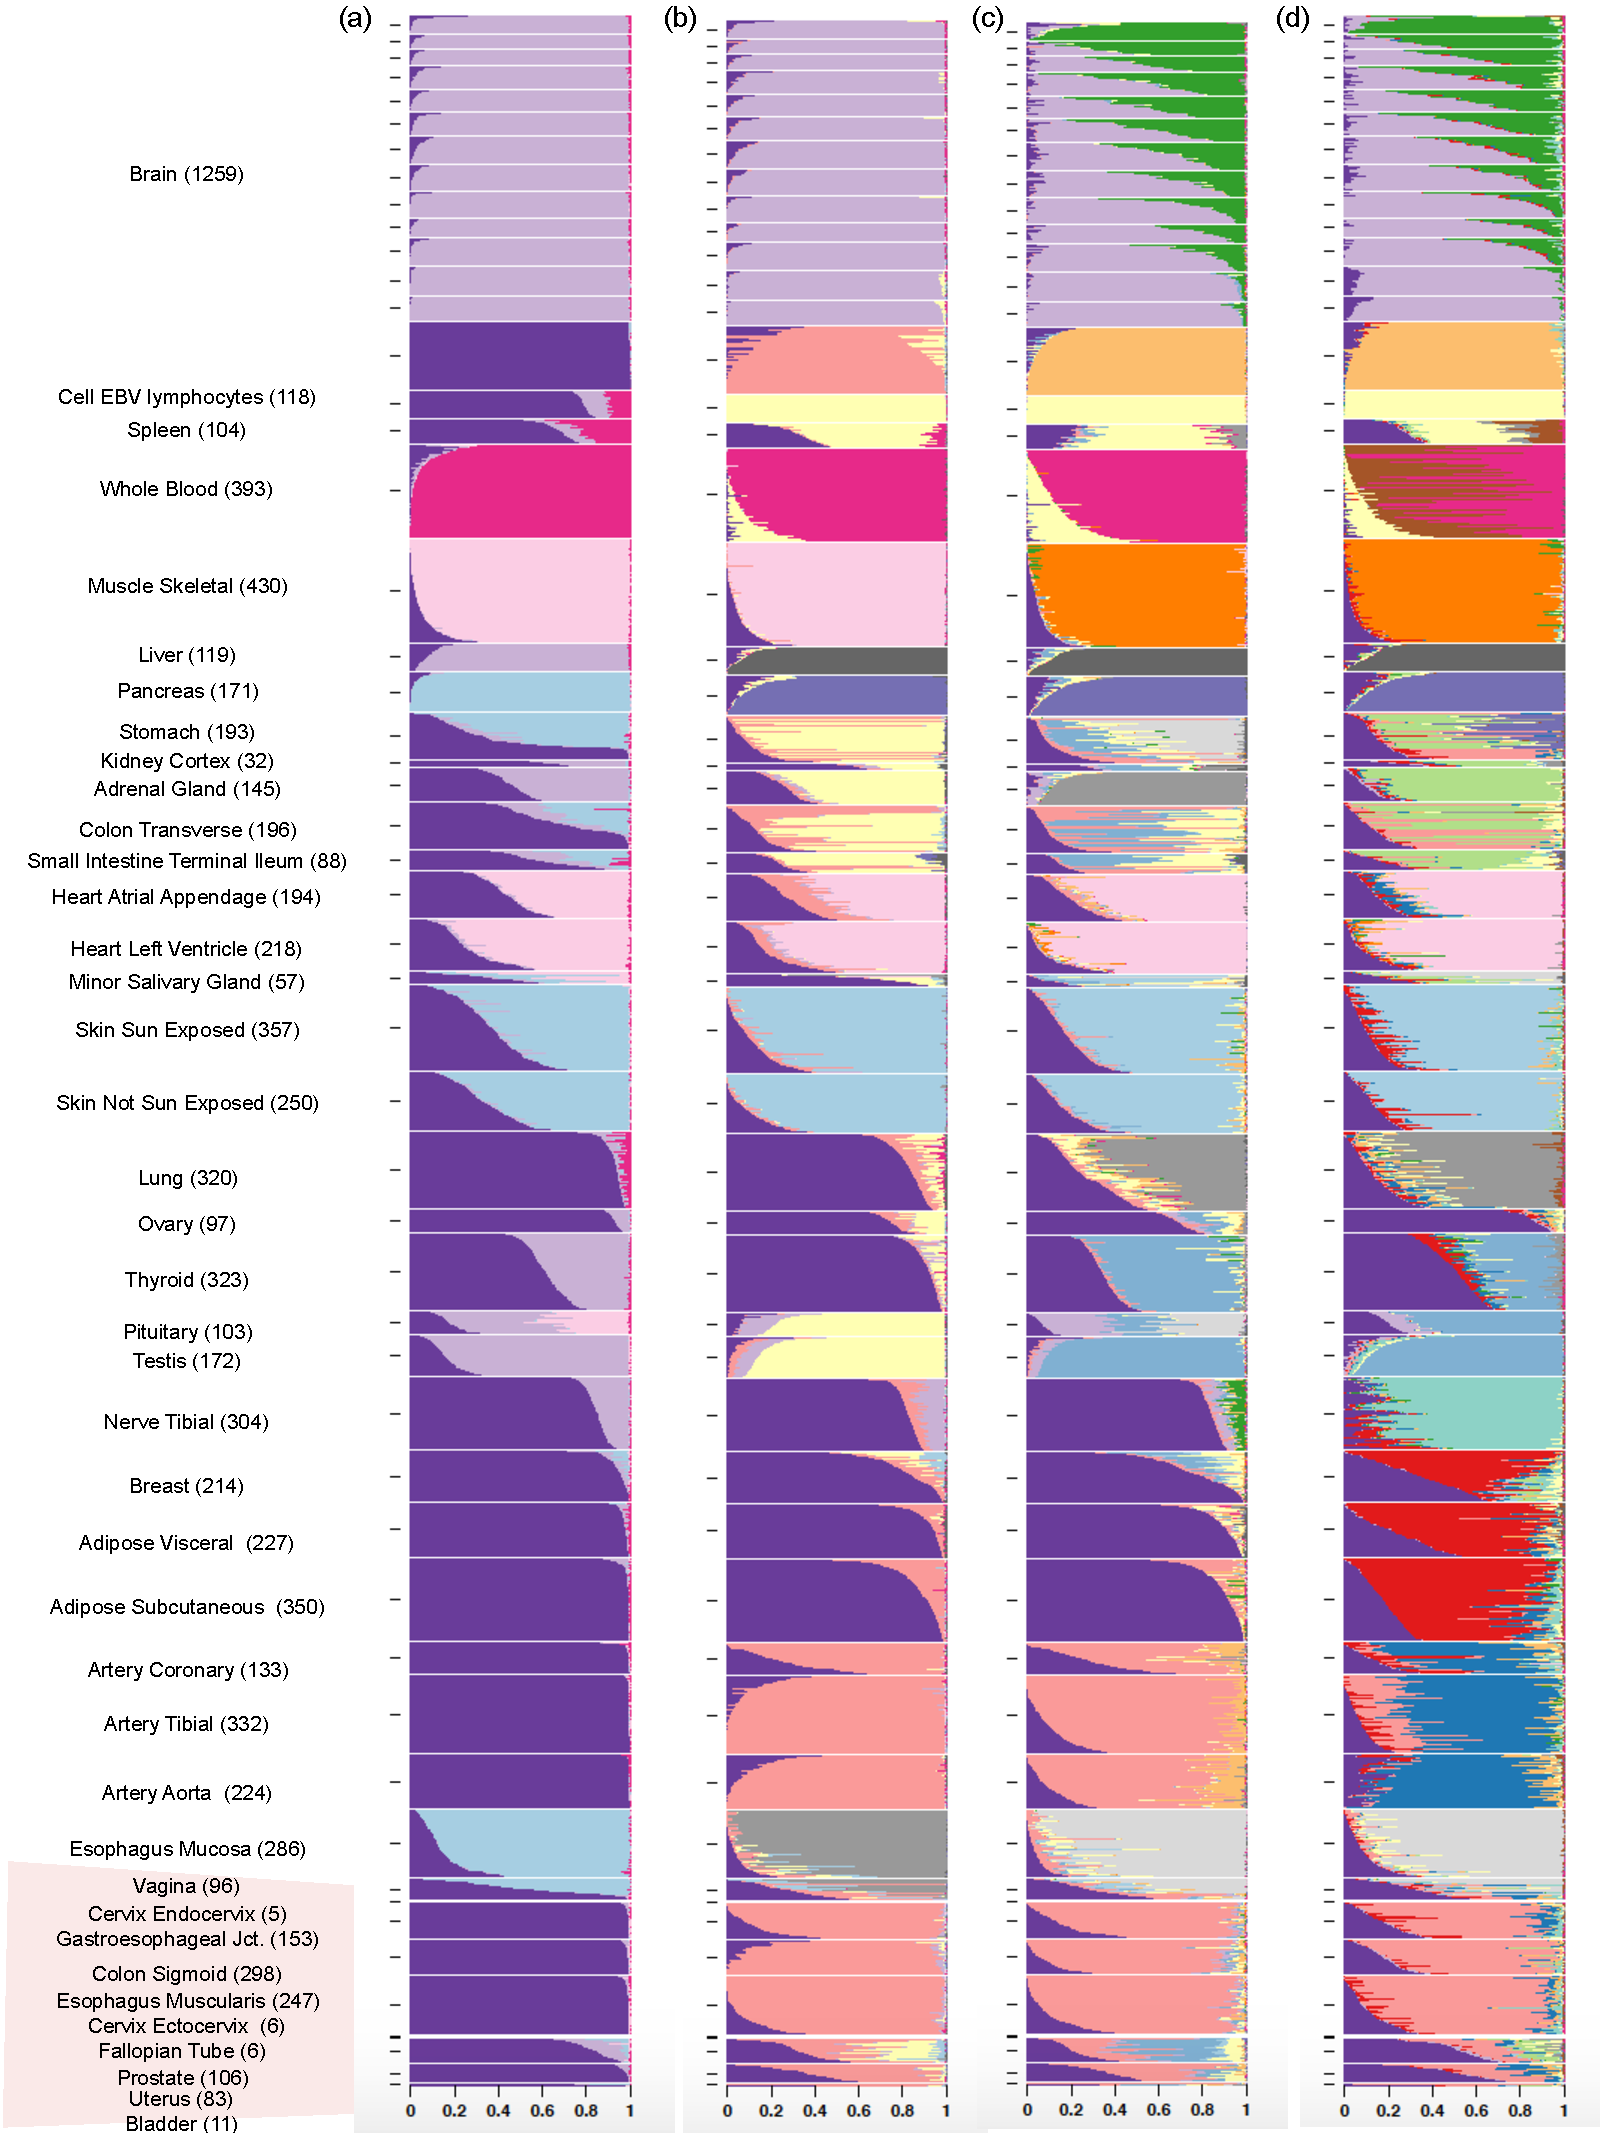
\includegraphics[height=7.5in, width=6.5in]{../../plots/gtex-figures/gtex-multiple-ks-04-30-2016}
\end{figure*}

\end{document}

\clearpage
% adopt PLoS genetics environment settings
\documentclass[10pt,letterpaper]{article}
\usepackage[top=0.85in,left=2.75in,footskip=0.75in]{geometry}

% Template for PLoS
% Version 3.2 March 2016

% General commands for the entire paper
%
% Use Unicode characters when possible
\usepackage[utf8x]{inputenc}
% amsmath package, useful for mathematical formulas
\usepackage{amsmath}
%\usepackage{natbib}
% amssymb package, useful for mathematical symbols
\usepackage{amssymb}
\usepackage{booktabs}
\usepackage{xspace}
\usepackage{hyperref}
% graphicx package, useful for including eps and pdf graphics
% include graphics with the command \includegraphics
\usepackage{graphicx}

% Use adjustwidth environment to exceed column width (see example table in text)
\usepackage{changepage}

% textcomp package and marvosym package for additional characters
\usepackage{textcomp,marvosym}

% fixltx2e package for \textsubscript
\usepackage{fixltx2e}

% cite package, to clean up citations in the main text. Do not remove.
\usepackage{cite}
\usepackage{caption}
\usepackage{subcaption}
\usepackage{rotating}

\usepackage{color}

% Use doublespacing - comment out for single spacing
%\usepackage{setspace}
%\doublespacing

% Text layout
\topmargin 0.0cm
\oddsidemargin 0.5cm
\evensidemargin 0.5cm
\textwidth 16cm
\textheight 21cm

\setlength{\parskip}{1em}

% Bold the 'Figure #' in the caption and separate it with a period
% Captions will be left justified
\usepackage[labelfont=bf,labelsep=period,justification=raggedright]{caption}

% Use the PLoS provided bibtex style
\bibliographystyle{/Users/stephens/Dropbox/Documents/stylefiles/plos2009}

% Remove brackets from numbering in List of References
\makeatletter
\renewcommand{\@biblabel}[1]{\quad#1.}
\makeatother

% Use nameref to cite supporting information files (see Supporting Information section for more info)
\usepackage{nameref,hyperref}

% line numbers
\usepackage[right]{lineno}

% ligatures disabled
\usepackage{microtype}
\DisableLigatures[f]{encoding = *, family = * }

% Leave date blank
\date{}

\pagestyle{myheadings}
%% ** EDIT HERE **
\usepackage{enumerate}
\usepackage{multirow}
\usepackage{url}
\usepackage{xr} %for cross-referencing
%% ** EDIT HERE **
%% PLEASE INCLUDE ALL MACROS BELOW
\newtheorem{algorithm}{Algorithm}
\newtheorem{proposition}{Proposition}
\newtheorem{restateproposition}{Proposition}
\newtheorem{lemma}{Lemma}
\newtheorem{corollary}{Corollary}
\newtheorem{result}{Result}
\newtheorem{note}{Note}
\newtheorem{definition}{Definition}

\def\KL{\text{KL}}


% Text layout
\raggedright
\setlength{\parindent}{0.5cm}
\textwidth 5.25in
\textheight 8.75in

% Bold the 'Figure #' in the caption and separate it from the title/caption with a period
% Captions will be left justified
\usepackage[aboveskip=1pt,labelfont=bf,labelsep=period,justification=raggedright,singlelinecheck=off]{caption}
\renewcommand{\figurename}{Fig}

%------ bibliography
% Use the PLoS provided BiBTeX style
\bibliographystyle{plos2015}
% Remove brackets from numbering in List of References
\makeatletter
\renewcommand{\@biblabel}[1]{\quad#1.}
\makeatother


% Header and Footer with logo
\usepackage{lastpage,fancyhdr,graphicx}
\usepackage{epstopdf}
\pagestyle{myheadings}
\pagestyle{fancy}
\fancyhf{}
\setlength{\headheight}{27.023pt}
\lhead{\includegraphics[width=2.0in]{PLOS-submission.eps}}
\rfoot{\thepage/\pageref{LastPage}}
\renewcommand{\footrule}{\hrule height 2pt \vspace{2mm}}
\fancyheadoffset[L]{2.25in}
\fancyfootoffset[L]{2.25in}
\lfoot{\sf PLOS}

%% Include all macros below

\newcommand{\lorem}{{\bf LOREM}}
\newcommand{\ipsum}{{\bf IPSUM}}

%% END MACROS SECTION

%% Author's settings
\def\KL{\text{KL}}


\begin{document}

\paragraph*{S2 Fig.}
\label{figS2}
{\bf Structure plot of GTEx V6 all tissue samples K=20 in 2 runs under the thinning parameters settings (a) $p_{thin}=0.01$ and (b) $p_{thin}=0.0001$.} The patterns in two plots closely correspond to the plot in Fig~1(a), though there are a few differences from the unthinned version.
\begin{figure*}[ht]
\centering
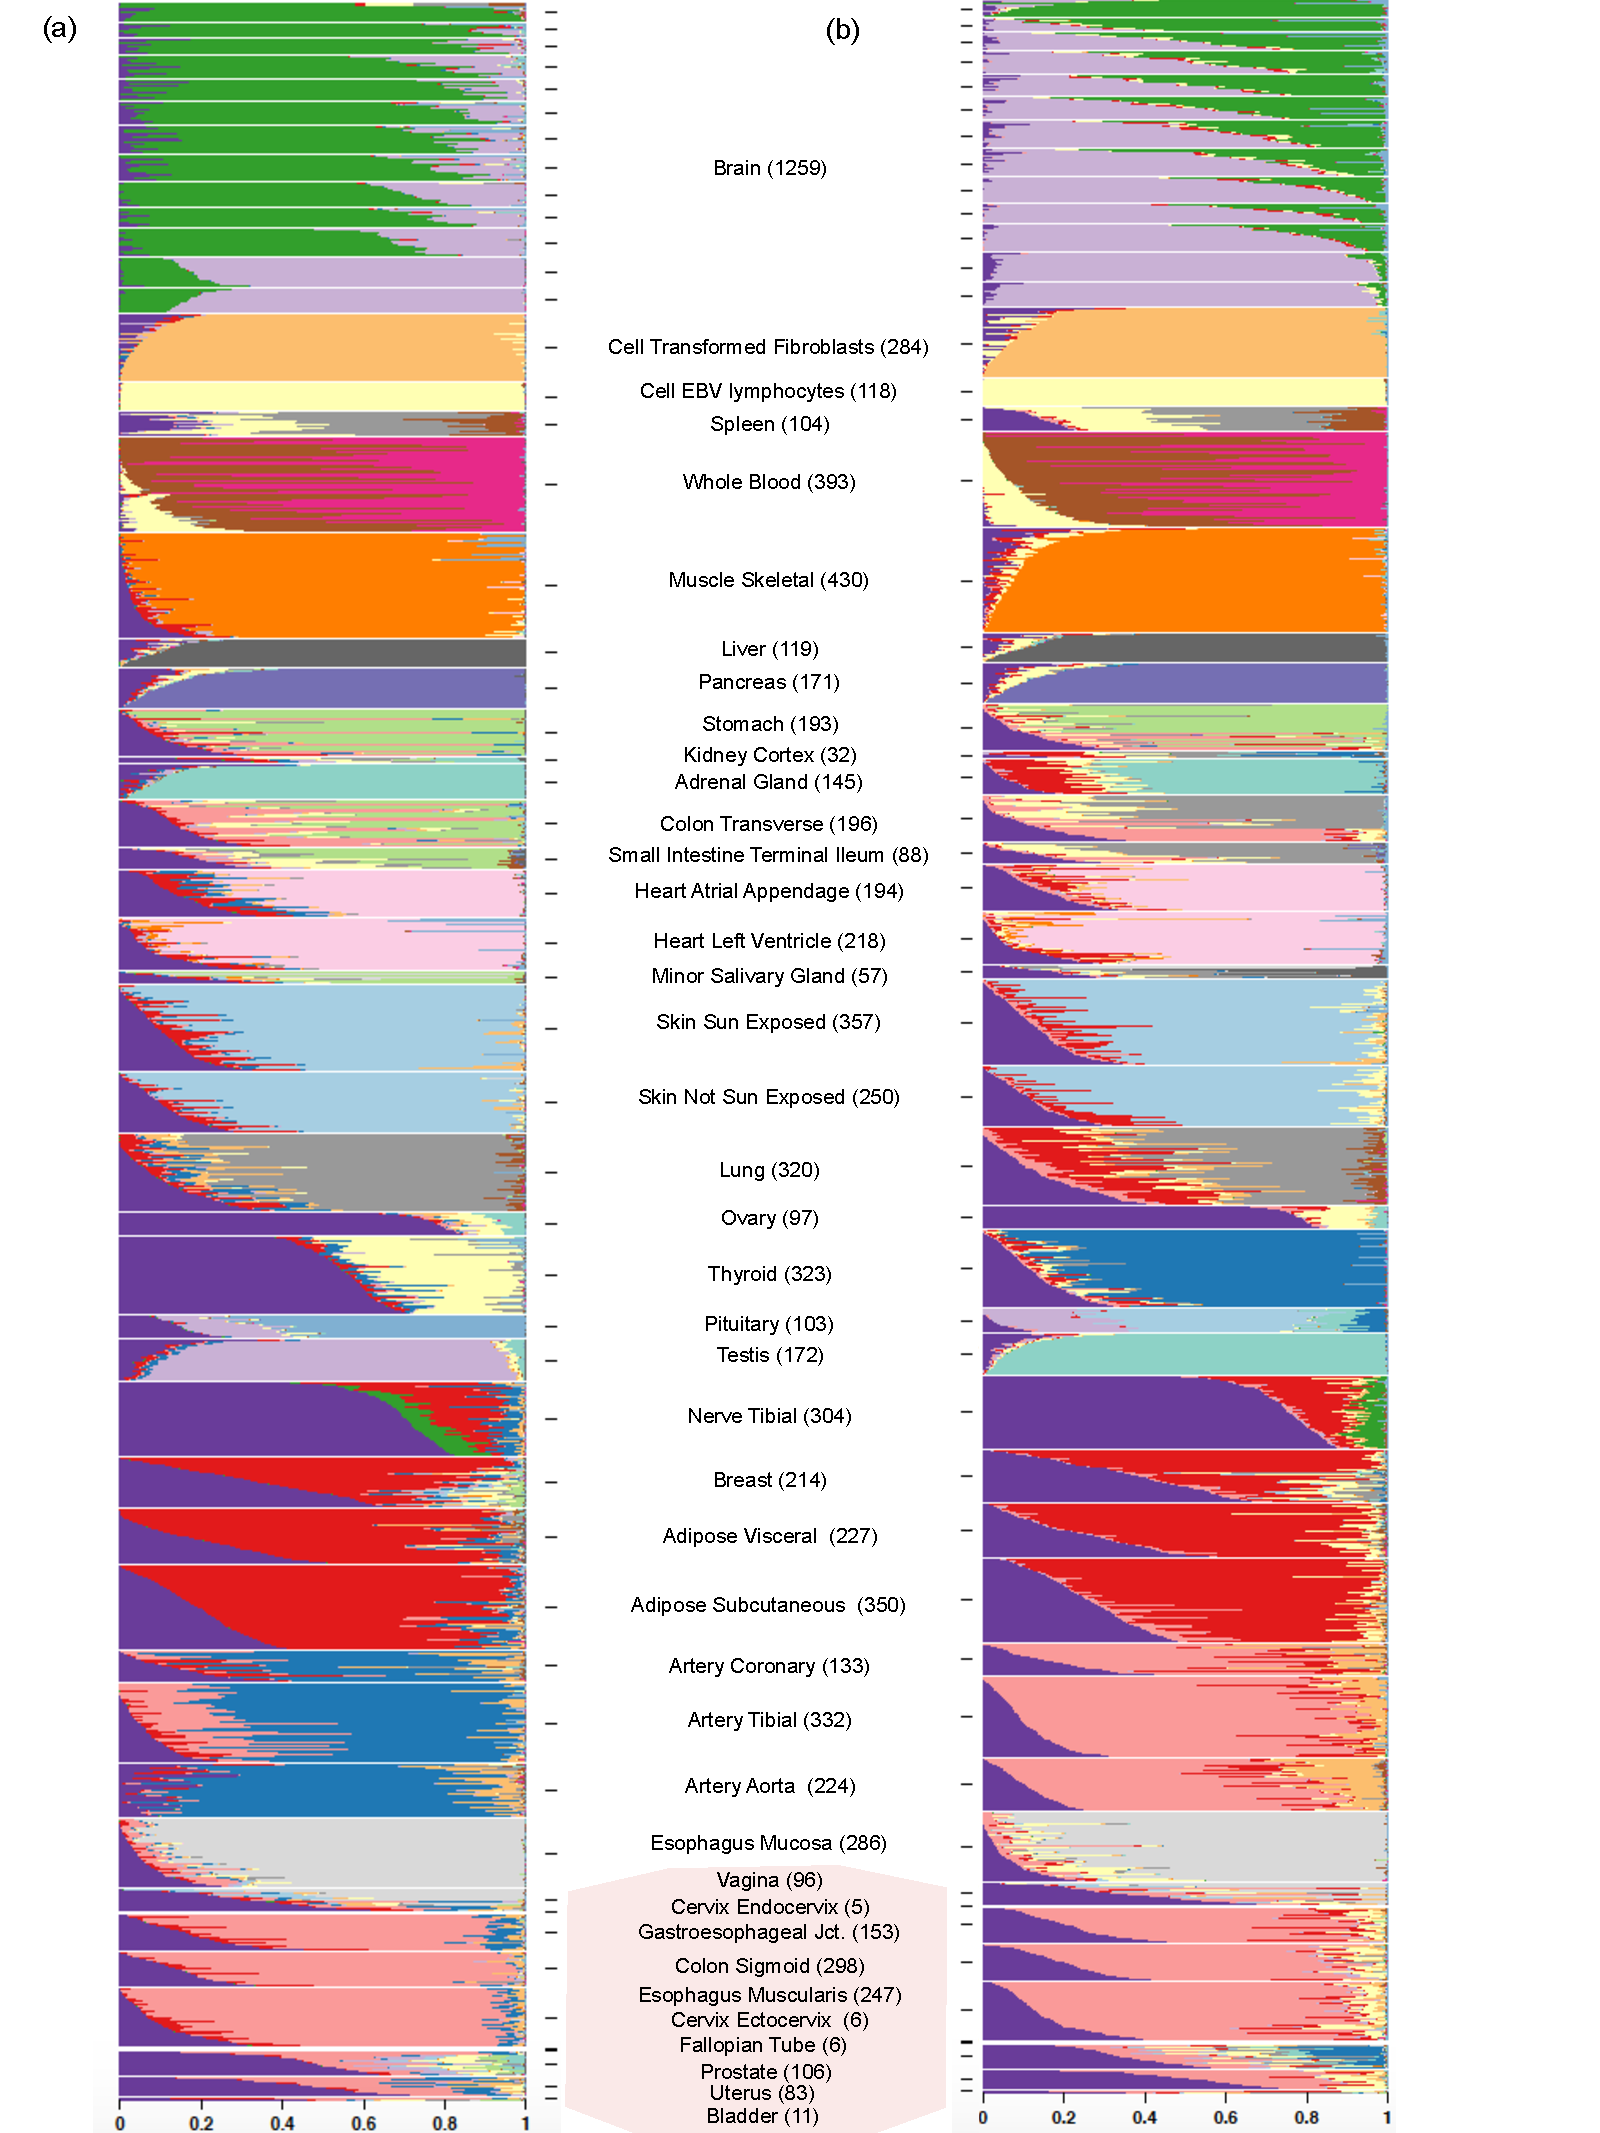
\includegraphics[height=7.5in, width=6.5in]{../../plots/gtex-figures/gtex_thinned_04_25_2016.pdf}
\end{figure*}
\clearpage

\end{document}

\clearpage
% adopt PLoS genetics environment settings
\documentclass[10pt,letterpaper]{article}
\usepackage[top=0.85in,left=2.75in,footskip=0.75in]{geometry}

% Template for PLoS
% Version 3.2 March 2016

% General commands for the entire paper
%
% Use Unicode characters when possible
\usepackage[utf8x]{inputenc}
% amsmath package, useful for mathematical formulas
\usepackage{amsmath}
%\usepackage{natbib}
% amssymb package, useful for mathematical symbols
\usepackage{amssymb}
\usepackage{booktabs}
\usepackage{xspace}
\usepackage{hyperref}
% graphicx package, useful for including eps and pdf graphics
% include graphics with the command \includegraphics
\usepackage{graphicx}

% Use adjustwidth environment to exceed column width (see example table in text)
\usepackage{changepage}

% textcomp package and marvosym package for additional characters
\usepackage{textcomp,marvosym}

% fixltx2e package for \textsubscript
\usepackage{fixltx2e}

% cite package, to clean up citations in the main text. Do not remove.
\usepackage{cite}
\usepackage{caption}
\usepackage{subcaption}
\usepackage{rotating}

\usepackage{color}

% Use doublespacing - comment out for single spacing
%\usepackage{setspace}
%\doublespacing

% Text layout
\topmargin 0.0cm
\oddsidemargin 0.5cm
\evensidemargin 0.5cm
\textwidth 16cm
\textheight 21cm

\setlength{\parskip}{1em}

% Bold the 'Figure #' in the caption and separate it with a period
% Captions will be left justified
\usepackage[labelfont=bf,labelsep=period,justification=raggedright]{caption}

% Use the PLoS provided bibtex style
\bibliographystyle{/Users/stephens/Dropbox/Documents/stylefiles/plos2009}

% Remove brackets from numbering in List of References
\makeatletter
\renewcommand{\@biblabel}[1]{\quad#1.}
\makeatother

% Use nameref to cite supporting information files (see Supporting Information section for more info)
\usepackage{nameref,hyperref}

% line numbers
\usepackage[right]{lineno}

% ligatures disabled
\usepackage{microtype}
\DisableLigatures[f]{encoding = *, family = * }

% Leave date blank
\date{}

\pagestyle{myheadings}
%% ** EDIT HERE **
\usepackage{enumerate}
\usepackage{multirow}
\usepackage{url}
\usepackage{xr} %for cross-referencing
%% ** EDIT HERE **
%% PLEASE INCLUDE ALL MACROS BELOW
\newtheorem{algorithm}{Algorithm}
\newtheorem{proposition}{Proposition}
\newtheorem{restateproposition}{Proposition}
\newtheorem{lemma}{Lemma}
\newtheorem{corollary}{Corollary}
\newtheorem{result}{Result}
\newtheorem{note}{Note}
\newtheorem{definition}{Definition}

\def\KL{\text{KL}}


% Text layout
\raggedright
\setlength{\parindent}{0.5cm}
\textwidth 5.25in
\textheight 8.75in

% Bold the 'Figure #' in the caption and separate it from the title/caption with a period
% Captions will be left justified
\usepackage[aboveskip=1pt,labelfont=bf,labelsep=period,justification=raggedright,singlelinecheck=off]{caption}
\renewcommand{\figurename}{Fig}

%------ bibliography
% Use the PLoS provided BiBTeX style
\bibliographystyle{plos2015}
% Remove brackets from numbering in List of References
\makeatletter
\renewcommand{\@biblabel}[1]{\quad#1.}
\makeatother


% Header and Footer with logo
\usepackage{lastpage,fancyhdr,graphicx}
\usepackage{epstopdf}
\pagestyle{myheadings}
\pagestyle{fancy}
\fancyhf{}
\setlength{\headheight}{27.023pt}
\lhead{\includegraphics[width=2.0in]{PLOS-submission.eps}}
\rfoot{\thepage/\pageref{LastPage}}
\renewcommand{\footrule}{\hrule height 2pt \vspace{2mm}}
\fancyheadoffset[L]{2.25in}
\fancyfootoffset[L]{2.25in}
\lfoot{\sf PLOS}

%% Include all macros below

\newcommand{\lorem}{{\bf LOREM}}
\newcommand{\ipsum}{{\bf IPSUM}}

%% END MACROS SECTION

%% Author's settings
\def\KL{\text{KL}}


% Text layout specific to Supplemental Materials
\topmargin 0.0cm
\oddsidemargin 0.5cm
\evensidemargin 0.5cm
\textwidth 16cm
\textheight 21cm

\setlength{\parskip}{1em}

\begin{document}

\paragraph*{S3 Fig.}
\label{figS3}
{\bf A comparison of ``accuracy" of hierarchical clustering vs. GoM on thinned GTEx data, with thinning parameters of $p_{thin}=0.01$ and $p_{thin}=0.001$.}  For each pair of tissue samples from the GTEx V6 data we assessed whether or not each clustering method (with $K=2$ clusters) separated the samples according to their tissue of origin, with successful separation indicated by a filled square. Thinning deteriorates accuracy compared with the unthinned data (Fig~2), but even then the model-based method remains more successful than the hierarchical clustering in separating the samples by tissue or origin.
 \begin{figure}[ht]
    \centering
     \begin{subfigure}[t]{0.5\textwidth}
        \centering
        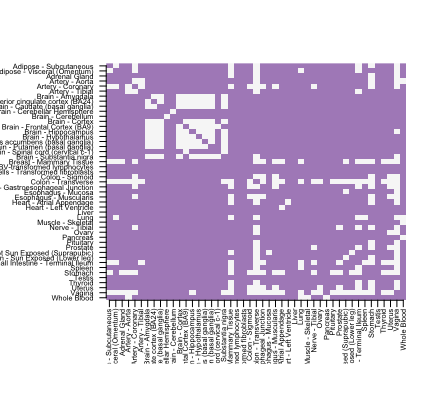
\includegraphics[height=2.5in]{../../plots/hierarchical_separation_thinned_0_001.png}
        \caption{hierarchy thin 0.01}
    \end{subfigure}%
    ~
    \begin{subfigure}[t]{0.5\textwidth}
        \centering
        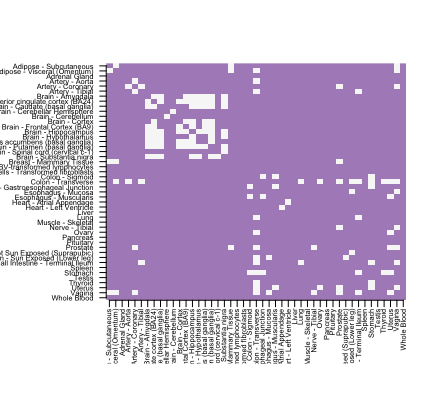
\includegraphics[height=2.5in]{../../plots/admixture_separation_thinned_0_01.png}
        \caption{GoM thin 0.01}
    \end{subfigure}\\

     \begin{subfigure}[t]{0.5\textwidth}
        \centering
        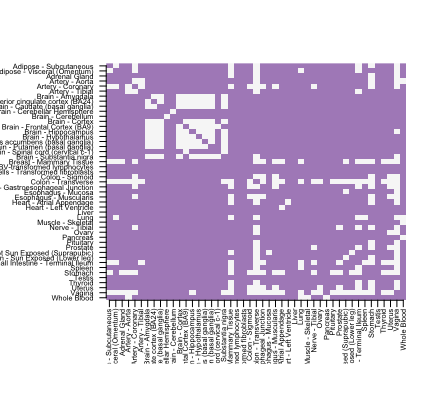
\includegraphics[height=2.5in]{../../plots/hierarchical_separation_thinned_0_001.png}
        \caption{hierarchy 0.001}
    \end{subfigure}%
    ~
    \begin{subfigure}[t]{0.5\textwidth}
        \centering
        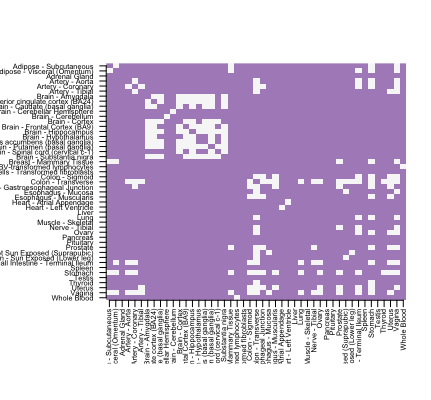
\includegraphics[height=2.5in]{../../plots/admixture_separation_thinned_0_001.png}
        \caption{GoM thin 0.001}
    \end{subfigure}\\
\end{figure}

\end{document}

\clearpage
% adopt PLoS genetics environment settings
\documentclass[10pt,letterpaper]{article}
\usepackage[top=0.85in,left=2.75in,footskip=0.75in]{geometry}

% Template for PLoS
% Version 3.2 March 2016

% General commands for the entire paper
%
% Use Unicode characters when possible
\usepackage[utf8x]{inputenc}
% amsmath package, useful for mathematical formulas
\usepackage{amsmath}
%\usepackage{natbib}
% amssymb package, useful for mathematical symbols
\usepackage{amssymb}
\usepackage{booktabs}
\usepackage{xspace}
\usepackage{hyperref}
% graphicx package, useful for including eps and pdf graphics
% include graphics with the command \includegraphics
\usepackage{graphicx}

% Use adjustwidth environment to exceed column width (see example table in text)
\usepackage{changepage}

% textcomp package and marvosym package for additional characters
\usepackage{textcomp,marvosym}

% fixltx2e package for \textsubscript
\usepackage{fixltx2e}

% cite package, to clean up citations in the main text. Do not remove.
\usepackage{cite}
\usepackage{caption}
\usepackage{subcaption}
\usepackage{rotating}

\usepackage{color}

% Use doublespacing - comment out for single spacing
%\usepackage{setspace}
%\doublespacing

% Text layout
\topmargin 0.0cm
\oddsidemargin 0.5cm
\evensidemargin 0.5cm
\textwidth 16cm
\textheight 21cm

\setlength{\parskip}{1em}

% Bold the 'Figure #' in the caption and separate it with a period
% Captions will be left justified
\usepackage[labelfont=bf,labelsep=period,justification=raggedright]{caption}

% Use the PLoS provided bibtex style
\bibliographystyle{/Users/stephens/Dropbox/Documents/stylefiles/plos2009}

% Remove brackets from numbering in List of References
\makeatletter
\renewcommand{\@biblabel}[1]{\quad#1.}
\makeatother

% Use nameref to cite supporting information files (see Supporting Information section for more info)
\usepackage{nameref,hyperref}

% line numbers
\usepackage[right]{lineno}

% ligatures disabled
\usepackage{microtype}
\DisableLigatures[f]{encoding = *, family = * }

% Leave date blank
\date{}

\pagestyle{myheadings}
%% ** EDIT HERE **
\usepackage{enumerate}
\usepackage{multirow}
\usepackage{url}
\usepackage{xr} %for cross-referencing
%% ** EDIT HERE **
%% PLEASE INCLUDE ALL MACROS BELOW
\newtheorem{algorithm}{Algorithm}
\newtheorem{proposition}{Proposition}
\newtheorem{restateproposition}{Proposition}
\newtheorem{lemma}{Lemma}
\newtheorem{corollary}{Corollary}
\newtheorem{result}{Result}
\newtheorem{note}{Note}
\newtheorem{definition}{Definition}

\def\KL{\text{KL}}


% Text layout
\raggedright
\setlength{\parindent}{0.5cm}
\textwidth 5.25in
\textheight 8.75in

% Bold the 'Figure #' in the caption and separate it from the title/caption with a period
% Captions will be left justified
\usepackage[aboveskip=1pt,labelfont=bf,labelsep=period,justification=raggedright,singlelinecheck=off]{caption}
\renewcommand{\figurename}{Fig}

%------ bibliography
% Use the PLoS provided BiBTeX style
\bibliographystyle{plos2015}
% Remove brackets from numbering in List of References
\makeatletter
\renewcommand{\@biblabel}[1]{\quad#1.}
\makeatother


% Header and Footer with logo
\usepackage{lastpage,fancyhdr,graphicx}
\usepackage{epstopdf}
\pagestyle{myheadings}
\pagestyle{fancy}
\fancyhf{}
\setlength{\headheight}{27.023pt}
\lhead{\includegraphics[width=2.0in]{PLOS-submission.eps}}
\rfoot{\thepage/\pageref{LastPage}}
\renewcommand{\footrule}{\hrule height 2pt \vspace{2mm}}
\fancyheadoffset[L]{2.25in}
\fancyfootoffset[L]{2.25in}
\lfoot{\sf PLOS}

%% Include all macros below

\newcommand{\lorem}{{\bf LOREM}}
\newcommand{\ipsum}{{\bf IPSUM}}

%% END MACROS SECTION

%% Author's settings
\def\KL{\text{KL}}


% Text layout specific to Supplemental Materials
\topmargin 0.0cm
\oddsidemargin 0.5cm
\evensidemargin 0.5cm
\textwidth 16cm
\textheight 21cm

\setlength{\parskip}{1em}

\begin{document}

\paragraph*{S4 Fig.}

\label{figS4}
{\bf GTEx data visualization of all tissue samples using (a) principle component analysis and (b) t-SNE
(c) Multidimensional scaling.}
Samples of matching tissue types are indicated by points of matching color.
\begin{figure}[ht]
\centering
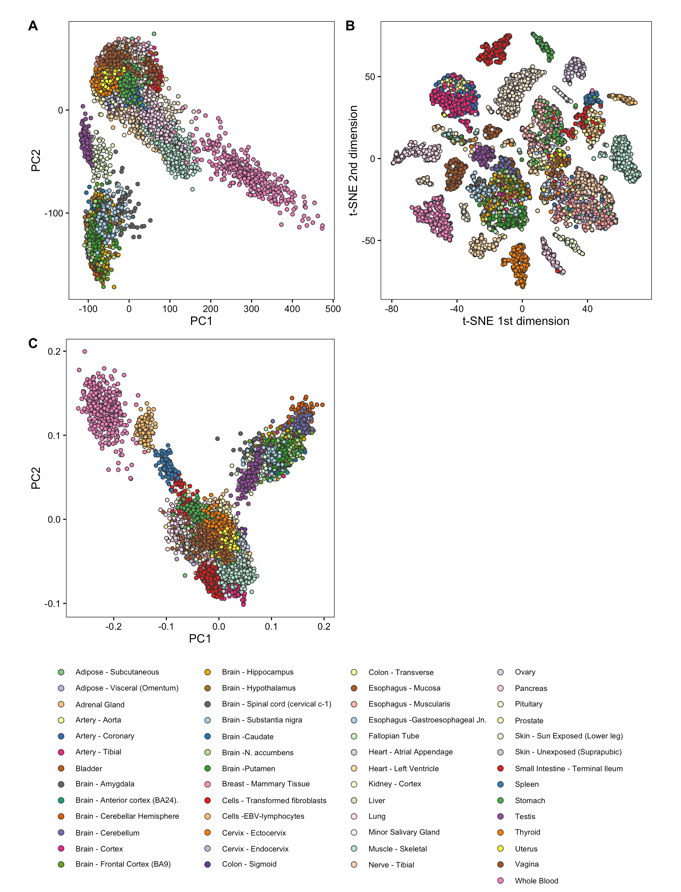
\includegraphics[height=6in, width=5in]{../../src/figure/gtex-other-methods.Rmd/gtex-with-legend.png}
\end{figure}

\end{document}

\clearpage
% adopt PLoS genetics environment settings
\documentclass[10pt,letterpaper]{article}
\usepackage[top=0.85in,left=2.75in,footskip=0.75in]{geometry}

% Template for PLoS
% Version 3.2 March 2016

% General commands for the entire paper
%
% Use Unicode characters when possible
\usepackage[utf8x]{inputenc}
% amsmath package, useful for mathematical formulas
\usepackage{amsmath}
%\usepackage{natbib}
% amssymb package, useful for mathematical symbols
\usepackage{amssymb}
\usepackage{booktabs}
\usepackage{xspace}
\usepackage{hyperref}
% graphicx package, useful for including eps and pdf graphics
% include graphics with the command \includegraphics
\usepackage{graphicx}

% Use adjustwidth environment to exceed column width (see example table in text)
\usepackage{changepage}

% textcomp package and marvosym package for additional characters
\usepackage{textcomp,marvosym}

% fixltx2e package for \textsubscript
\usepackage{fixltx2e}

% cite package, to clean up citations in the main text. Do not remove.
\usepackage{cite}
\usepackage{caption}
\usepackage{subcaption}
\usepackage{rotating}

\usepackage{color}

% Use doublespacing - comment out for single spacing
%\usepackage{setspace}
%\doublespacing

% Text layout
\topmargin 0.0cm
\oddsidemargin 0.5cm
\evensidemargin 0.5cm
\textwidth 16cm
\textheight 21cm

\setlength{\parskip}{1em}

% Bold the 'Figure #' in the caption and separate it with a period
% Captions will be left justified
\usepackage[labelfont=bf,labelsep=period,justification=raggedright]{caption}

% Use the PLoS provided bibtex style
\bibliographystyle{/Users/stephens/Dropbox/Documents/stylefiles/plos2009}

% Remove brackets from numbering in List of References
\makeatletter
\renewcommand{\@biblabel}[1]{\quad#1.}
\makeatother

% Use nameref to cite supporting information files (see Supporting Information section for more info)
\usepackage{nameref,hyperref}

% line numbers
\usepackage[right]{lineno}

% ligatures disabled
\usepackage{microtype}
\DisableLigatures[f]{encoding = *, family = * }

% Leave date blank
\date{}

\pagestyle{myheadings}
%% ** EDIT HERE **
\usepackage{enumerate}
\usepackage{multirow}
\usepackage{url}
\usepackage{xr} %for cross-referencing
%% ** EDIT HERE **
%% PLEASE INCLUDE ALL MACROS BELOW
\newtheorem{algorithm}{Algorithm}
\newtheorem{proposition}{Proposition}
\newtheorem{restateproposition}{Proposition}
\newtheorem{lemma}{Lemma}
\newtheorem{corollary}{Corollary}
\newtheorem{result}{Result}
\newtheorem{note}{Note}
\newtheorem{definition}{Definition}

\def\KL{\text{KL}}


% Text layout
\raggedright
\setlength{\parindent}{0.5cm}
\textwidth 5.25in
\textheight 8.75in

% Bold the 'Figure #' in the caption and separate it from the title/caption with a period
% Captions will be left justified
\usepackage[aboveskip=1pt,labelfont=bf,labelsep=period,justification=raggedright,singlelinecheck=off]{caption}
\renewcommand{\figurename}{Fig}

%------ bibliography
% Use the PLoS provided BiBTeX style
\bibliographystyle{plos2015}
% Remove brackets from numbering in List of References
\makeatletter
\renewcommand{\@biblabel}[1]{\quad#1.}
\makeatother


% Header and Footer with logo
\usepackage{lastpage,fancyhdr,graphicx}
\usepackage{epstopdf}
\pagestyle{myheadings}
\pagestyle{fancy}
\fancyhf{}
\setlength{\headheight}{27.023pt}
\lhead{\includegraphics[width=2.0in]{PLOS-submission.eps}}
\rfoot{\thepage/\pageref{LastPage}}
\renewcommand{\footrule}{\hrule height 2pt \vspace{2mm}}
\fancyheadoffset[L]{2.25in}
\fancyfootoffset[L]{2.25in}
\lfoot{\sf PLOS}

%% Include all macros below

\newcommand{\lorem}{{\bf LOREM}}
\newcommand{\ipsum}{{\bf IPSUM}}

%% END MACROS SECTION

%% Author's settings
\def\KL{\text{KL}}


% Text layout specific to Supplemental Materials
\topmargin 0.0cm
\oddsidemargin 0.5cm
\evensidemargin 0.5cm
\textwidth 16cm
\textheight 21cm

\setlength{\parskip}{1em}

\begin{document}

\paragraph*{S5 Fig.}

\label{figS5}
{\bf Mouse embryo single cell sample visualization using (a) principle component analysis and (b) t-SNE
(c) Multidimensional scaling.}
Single cell samples collected at the same developmental stage are indicated by points of matching color.
\begin{figure*}[ht]
\centering
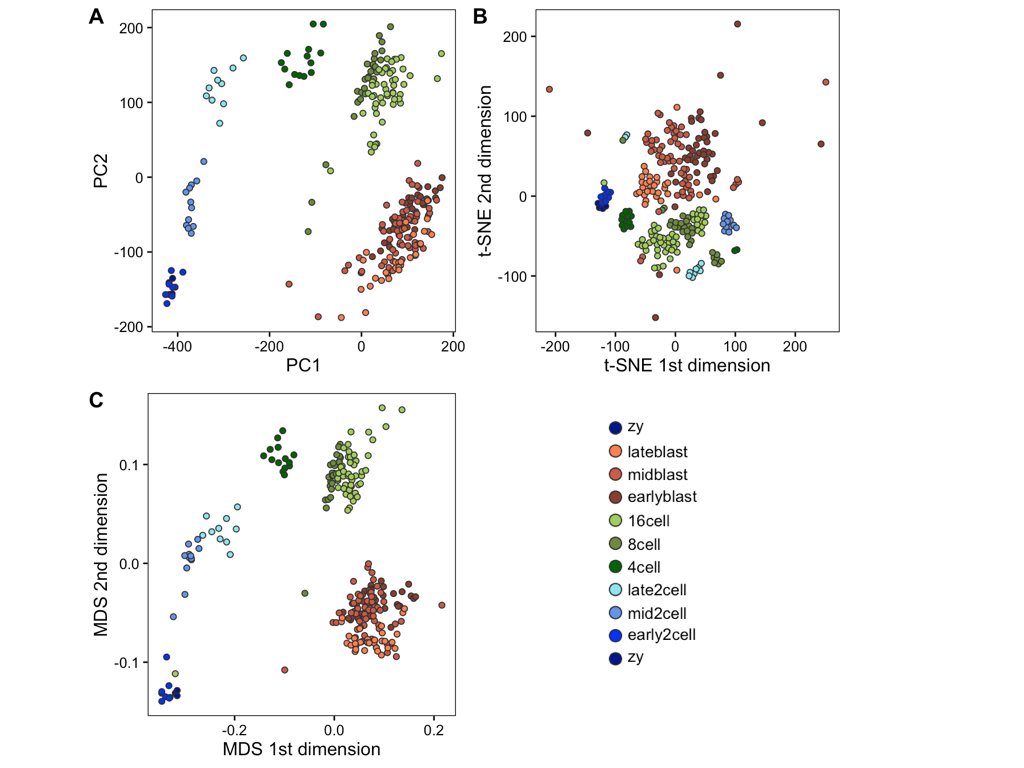
\includegraphics[height=4in, width=6in]{../../src/figure/deng-other-methods.Rmd/deng-with-legend.jpeg}
\end{figure*}

\end{document}

\clearpage
% adopt PLoS genetics environment settings
\documentclass[10pt,letterpaper]{article}
\usepackage[top=0.85in,left=2.75in,footskip=0.75in]{geometry}

% Template for PLoS
% Version 3.2 March 2016

% General commands for the entire paper
%
% Use Unicode characters when possible
\usepackage[utf8x]{inputenc}
% amsmath package, useful for mathematical formulas
\usepackage{amsmath}
%\usepackage{natbib}
% amssymb package, useful for mathematical symbols
\usepackage{amssymb}
\usepackage{booktabs}
\usepackage{xspace}
\usepackage{hyperref}
% graphicx package, useful for including eps and pdf graphics
% include graphics with the command \includegraphics
\usepackage{graphicx}

% Use adjustwidth environment to exceed column width (see example table in text)
\usepackage{changepage}

% textcomp package and marvosym package for additional characters
\usepackage{textcomp,marvosym}

% fixltx2e package for \textsubscript
\usepackage{fixltx2e}

% cite package, to clean up citations in the main text. Do not remove.
\usepackage{cite}
\usepackage{caption}
\usepackage{subcaption}
\usepackage{rotating}

\usepackage{color}

% Use doublespacing - comment out for single spacing
%\usepackage{setspace}
%\doublespacing

% Text layout
\topmargin 0.0cm
\oddsidemargin 0.5cm
\evensidemargin 0.5cm
\textwidth 16cm
\textheight 21cm

\setlength{\parskip}{1em}

% Bold the 'Figure #' in the caption and separate it with a period
% Captions will be left justified
\usepackage[labelfont=bf,labelsep=period,justification=raggedright]{caption}

% Use the PLoS provided bibtex style
\bibliographystyle{/Users/stephens/Dropbox/Documents/stylefiles/plos2009}

% Remove brackets from numbering in List of References
\makeatletter
\renewcommand{\@biblabel}[1]{\quad#1.}
\makeatother

% Use nameref to cite supporting information files (see Supporting Information section for more info)
\usepackage{nameref,hyperref}

% line numbers
\usepackage[right]{lineno}

% ligatures disabled
\usepackage{microtype}
\DisableLigatures[f]{encoding = *, family = * }

% Leave date blank
\date{}

\pagestyle{myheadings}
%% ** EDIT HERE **
\usepackage{enumerate}
\usepackage{multirow}
\usepackage{url}
\usepackage{xr} %for cross-referencing
%% ** EDIT HERE **
%% PLEASE INCLUDE ALL MACROS BELOW
\newtheorem{algorithm}{Algorithm}
\newtheorem{proposition}{Proposition}
\newtheorem{restateproposition}{Proposition}
\newtheorem{lemma}{Lemma}
\newtheorem{corollary}{Corollary}
\newtheorem{result}{Result}
\newtheorem{note}{Note}
\newtheorem{definition}{Definition}

\def\KL{\text{KL}}


% Text layout
\raggedright
\setlength{\parindent}{0.5cm}
\textwidth 5.25in
\textheight 8.75in

% Bold the 'Figure #' in the caption and separate it from the title/caption with a period
% Captions will be left justified
\usepackage[aboveskip=1pt,labelfont=bf,labelsep=period,justification=raggedright,singlelinecheck=off]{caption}
\renewcommand{\figurename}{Fig}

%------ bibliography
% Use the PLoS provided BiBTeX style
\bibliographystyle{plos2015}
% Remove brackets from numbering in List of References
\makeatletter
\renewcommand{\@biblabel}[1]{\quad#1.}
\makeatother


% Header and Footer with logo
\usepackage{lastpage,fancyhdr,graphicx}
\usepackage{epstopdf}
\pagestyle{myheadings}
\pagestyle{fancy}
\fancyhf{}
\setlength{\headheight}{27.023pt}
\lhead{\includegraphics[width=2.0in]{PLOS-submission.eps}}
\rfoot{\thepage/\pageref{LastPage}}
\renewcommand{\footrule}{\hrule height 2pt \vspace{2mm}}
\fancyheadoffset[L]{2.25in}
\fancyfootoffset[L]{2.25in}
\lfoot{\sf PLOS}

%% Include all macros below

\newcommand{\lorem}{{\bf LOREM}}
\newcommand{\ipsum}{{\bf IPSUM}}

%% END MACROS SECTION

%% Author's settings
\def\KL{\text{KL}}


% Text layout specific to Supplemental Materials
\topmargin 0.0cm
\oddsidemargin 0.5cm
\evensidemargin 0.5cm
\textwidth 16cm
\textheight 21cm

\setlength{\parskip}{1em}

\begin{document}

\paragraph*{S6 Fig.}
\label{figS6}
{\bf A comparison of ``accuracy" of hierarchical clustering vs. GoM on thinned GTEx data, with thinning parameters of $p_{thin}=0.01$ and $p_{thin}=0.001$.}  For each pair of tissue samples from the GTEx V6 data we assessed whether or not each clustering method (with $K=2$ clusters) separated the samples according to their tissue of origin, with successful separation indicated by a filled square. Thinning deteriorates accuracy compared with the unthinned data (Fig~2), but even then the model-based method remains more successful than the hierarchical clustering in separating the samples by tissue or origin.
\begin{figure}[ht]
\centering
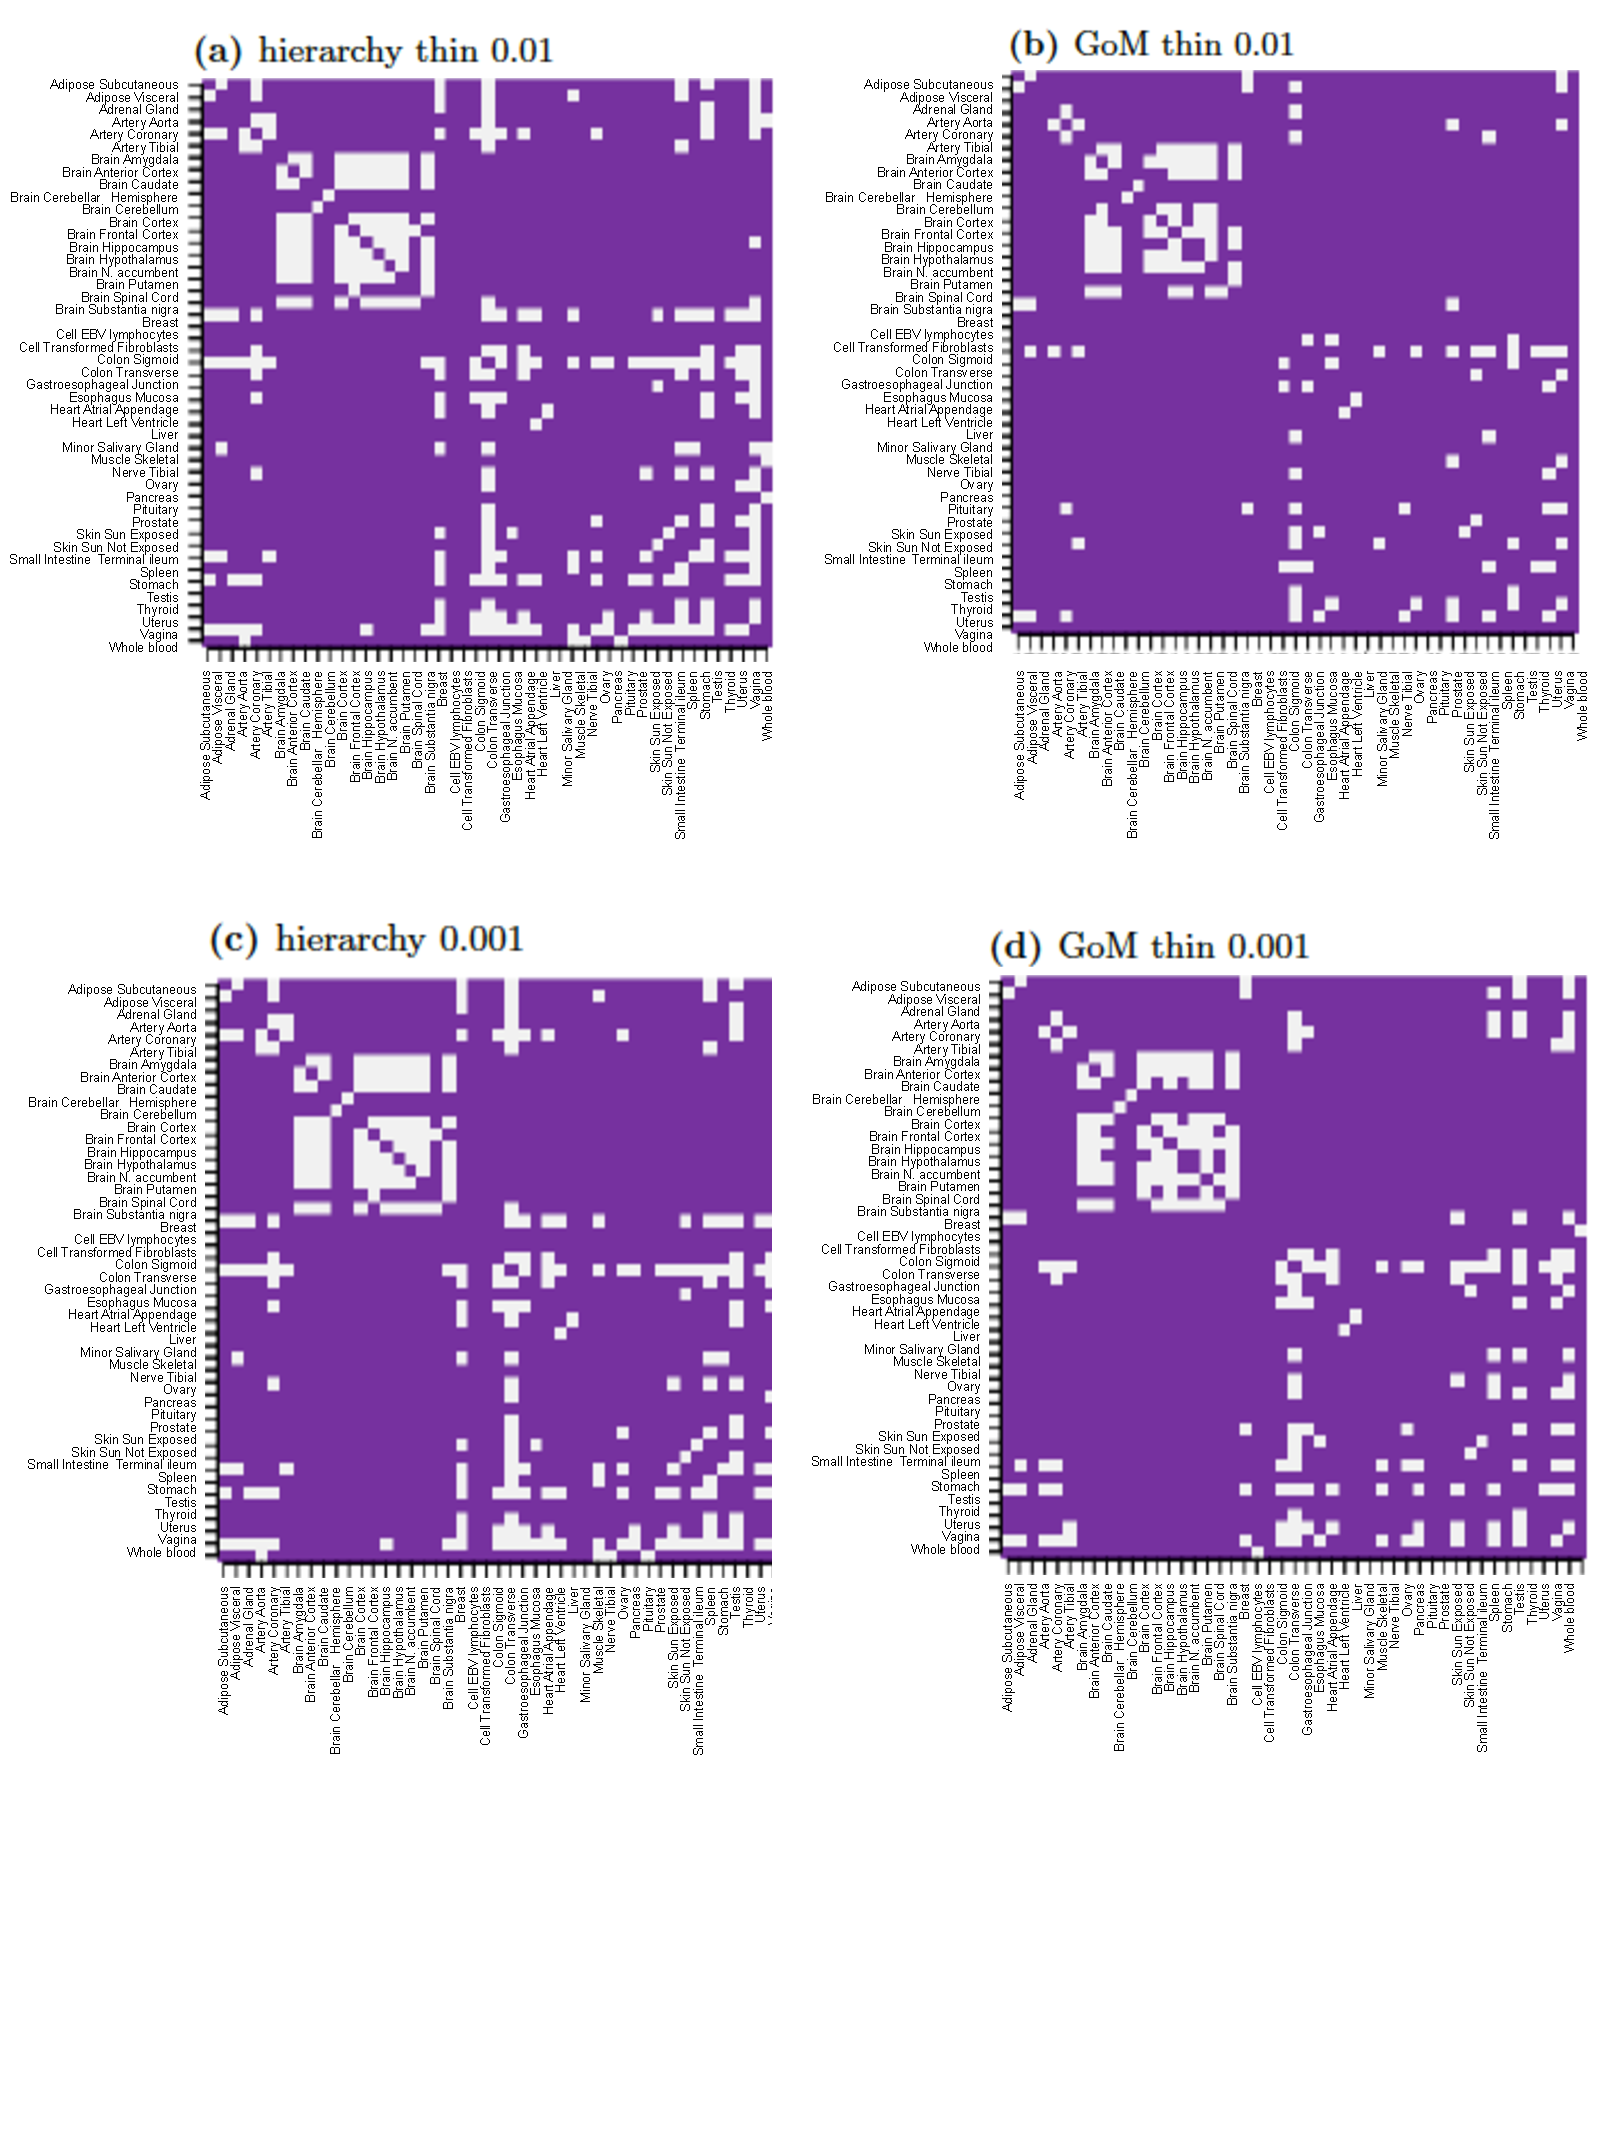
\includegraphics[height=9in, width=7in]{../figs-edits/figS6-edits.pdf}
\end{figure}
\end{document}

\clearpage
% adopt PLoS genetics environment settings
\documentclass[10pt,letterpaper]{article}
\usepackage[top=0.85in,left=2.75in,footskip=0.75in]{geometry}

% Template for PLoS
% Version 3.2 March 2016

% General commands for the entire paper
%
% Use Unicode characters when possible
\usepackage[utf8x]{inputenc}
% amsmath package, useful for mathematical formulas
\usepackage{amsmath}
%\usepackage{natbib}
% amssymb package, useful for mathematical symbols
\usepackage{amssymb}
\usepackage{booktabs}
\usepackage{xspace}
\usepackage{hyperref}
% graphicx package, useful for including eps and pdf graphics
% include graphics with the command \includegraphics
\usepackage{graphicx}

% Use adjustwidth environment to exceed column width (see example table in text)
\usepackage{changepage}

% textcomp package and marvosym package for additional characters
\usepackage{textcomp,marvosym}

% fixltx2e package for \textsubscript
\usepackage{fixltx2e}

% cite package, to clean up citations in the main text. Do not remove.
\usepackage{cite}
\usepackage{caption}
\usepackage{subcaption}
\usepackage{rotating}

\usepackage{color}

% Use doublespacing - comment out for single spacing
%\usepackage{setspace}
%\doublespacing

% Text layout
\topmargin 0.0cm
\oddsidemargin 0.5cm
\evensidemargin 0.5cm
\textwidth 16cm
\textheight 21cm

\setlength{\parskip}{1em}

% Bold the 'Figure #' in the caption and separate it with a period
% Captions will be left justified
\usepackage[labelfont=bf,labelsep=period,justification=raggedright]{caption}

% Use the PLoS provided bibtex style
\bibliographystyle{/Users/stephens/Dropbox/Documents/stylefiles/plos2009}

% Remove brackets from numbering in List of References
\makeatletter
\renewcommand{\@biblabel}[1]{\quad#1.}
\makeatother

% Use nameref to cite supporting information files (see Supporting Information section for more info)
\usepackage{nameref,hyperref}

% line numbers
\usepackage[right]{lineno}

% ligatures disabled
\usepackage{microtype}
\DisableLigatures[f]{encoding = *, family = * }

% Leave date blank
\date{}

\pagestyle{myheadings}
%% ** EDIT HERE **
\usepackage{enumerate}
\usepackage{multirow}
\usepackage{url}
\usepackage{xr} %for cross-referencing
%% ** EDIT HERE **
%% PLEASE INCLUDE ALL MACROS BELOW
\newtheorem{algorithm}{Algorithm}
\newtheorem{proposition}{Proposition}
\newtheorem{restateproposition}{Proposition}
\newtheorem{lemma}{Lemma}
\newtheorem{corollary}{Corollary}
\newtheorem{result}{Result}
\newtheorem{note}{Note}
\newtheorem{definition}{Definition}

\def\KL{\text{KL}}


% Text layout
\raggedright
\setlength{\parindent}{0.5cm}
\textwidth 5.25in
\textheight 8.75in

% Bold the 'Figure #' in the caption and separate it from the title/caption with a period
% Captions will be left justified
\usepackage[aboveskip=1pt,labelfont=bf,labelsep=period,justification=raggedright,singlelinecheck=off]{caption}
\renewcommand{\figurename}{Fig}

%------ bibliography
% Use the PLoS provided BiBTeX style
\bibliographystyle{plos2015}
% Remove brackets from numbering in List of References
\makeatletter
\renewcommand{\@biblabel}[1]{\quad#1.}
\makeatother


% Header and Footer with logo
\usepackage{lastpage,fancyhdr,graphicx}
\usepackage{epstopdf}
\pagestyle{myheadings}
\pagestyle{fancy}
\fancyhf{}
\setlength{\headheight}{27.023pt}
\lhead{\includegraphics[width=2.0in]{PLOS-submission.eps}}
\rfoot{\thepage/\pageref{LastPage}}
\renewcommand{\footrule}{\hrule height 2pt \vspace{2mm}}
\fancyheadoffset[L]{2.25in}
\fancyfootoffset[L]{2.25in}
\lfoot{\sf PLOS}

%% Include all macros below

\newcommand{\lorem}{{\bf LOREM}}
\newcommand{\ipsum}{{\bf IPSUM}}

%% END MACROS SECTION

%% Author's settings
\def\KL{\text{KL}}


% Text layout specific to Supplemental Materials
\topmargin 0.0cm
\oddsidemargin 0.5cm
\evensidemargin 0.5cm
\textwidth 16cm
\textheight 21cm

\setlength{\parskip}{1em}

\begin{document}

\paragraph*{S7 Fig.}

\label{figS7}
{\bf GTEx brain tissue samples visualization using (A) principle component analysis, (B) t-SNE, and (C) Multidimensional scaling.}
The colors represent the 13 different brain tissue types. In (A) and (B), the majority of the tissue samples are distinct from Cerebellum tissue samples (the cluster of samples located on the right side of the plot). While, in (C), most tissue samples are located at the enter of the plot and are similar to each other in the t-SNE dimensions.

\begin{figure}[ht]
\centering
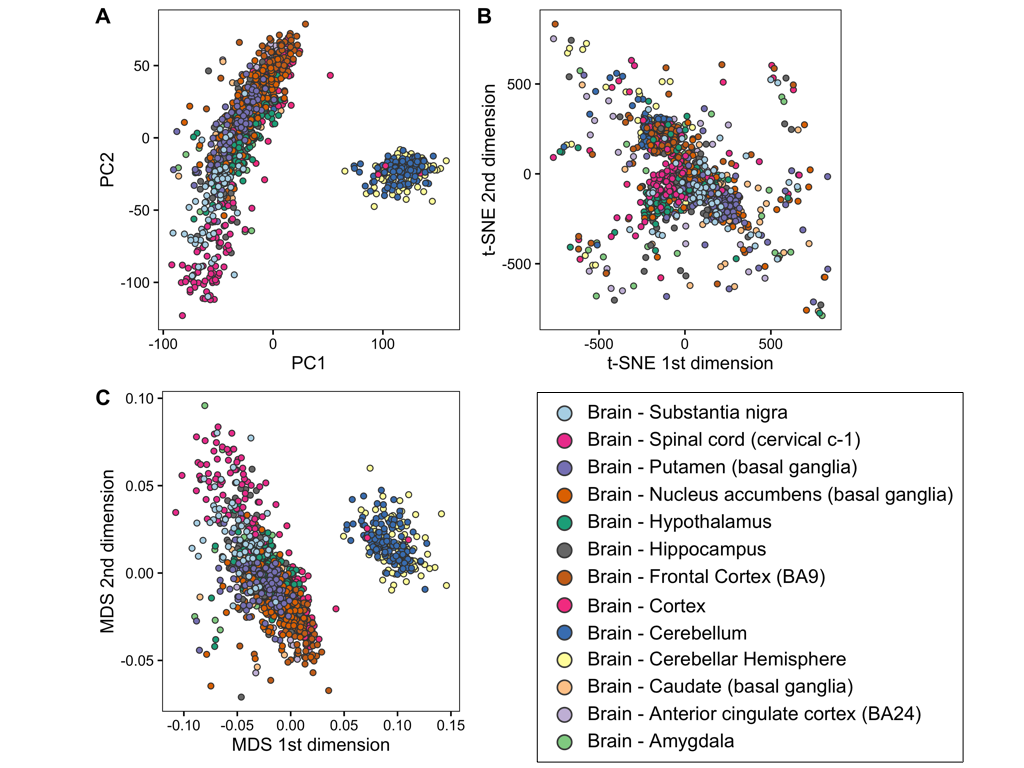
\includegraphics[height=4in, width=6in]{../../src/figure/gtex-brain-other-methods.Rmd/gtex-brain-with-legend.png}
\end{figure}

\end{document}

\clearpage
% adopt PLoS genetics environment settings
\documentclass[10pt,letterpaper]{article}
\usepackage[top=0.85in,left=2.75in,footskip=0.75in]{geometry}

% Template for PLoS
% Version 3.2 March 2016

% General commands for the entire paper
%
% Use Unicode characters when possible
\usepackage[utf8x]{inputenc}
% amsmath package, useful for mathematical formulas
\usepackage{amsmath}
%\usepackage{natbib}
% amssymb package, useful for mathematical symbols
\usepackage{amssymb}
\usepackage{booktabs}
\usepackage{xspace}
\usepackage{hyperref}
% graphicx package, useful for including eps and pdf graphics
% include graphics with the command \includegraphics
\usepackage{graphicx}

% Use adjustwidth environment to exceed column width (see example table in text)
\usepackage{changepage}

% textcomp package and marvosym package for additional characters
\usepackage{textcomp,marvosym}

% fixltx2e package for \textsubscript
\usepackage{fixltx2e}

% cite package, to clean up citations in the main text. Do not remove.
\usepackage{cite}
\usepackage{caption}
\usepackage{subcaption}
\usepackage{rotating}

\usepackage{color}

% Use doublespacing - comment out for single spacing
%\usepackage{setspace}
%\doublespacing

% Text layout
\topmargin 0.0cm
\oddsidemargin 0.5cm
\evensidemargin 0.5cm
\textwidth 16cm
\textheight 21cm

\setlength{\parskip}{1em}

% Bold the 'Figure #' in the caption and separate it with a period
% Captions will be left justified
\usepackage[labelfont=bf,labelsep=period,justification=raggedright]{caption}

% Use the PLoS provided bibtex style
\bibliographystyle{/Users/stephens/Dropbox/Documents/stylefiles/plos2009}

% Remove brackets from numbering in List of References
\makeatletter
\renewcommand{\@biblabel}[1]{\quad#1.}
\makeatother

% Use nameref to cite supporting information files (see Supporting Information section for more info)
\usepackage{nameref,hyperref}

% line numbers
\usepackage[right]{lineno}

% ligatures disabled
\usepackage{microtype}
\DisableLigatures[f]{encoding = *, family = * }

% Leave date blank
\date{}

\pagestyle{myheadings}
%% ** EDIT HERE **
\usepackage{enumerate}
\usepackage{multirow}
\usepackage{url}
\usepackage{xr} %for cross-referencing
%% ** EDIT HERE **
%% PLEASE INCLUDE ALL MACROS BELOW
\newtheorem{algorithm}{Algorithm}
\newtheorem{proposition}{Proposition}
\newtheorem{restateproposition}{Proposition}
\newtheorem{lemma}{Lemma}
\newtheorem{corollary}{Corollary}
\newtheorem{result}{Result}
\newtheorem{note}{Note}
\newtheorem{definition}{Definition}

\def\KL{\text{KL}}


% Text layout
\raggedright
\setlength{\parindent}{0.5cm}
\textwidth 5.25in
\textheight 8.75in

% Bold the 'Figure #' in the caption and separate it from the title/caption with a period
% Captions will be left justified
\usepackage[aboveskip=1pt,labelfont=bf,labelsep=period,justification=raggedright,singlelinecheck=off]{caption}
\renewcommand{\figurename}{Fig}

%------ bibliography
% Use the PLoS provided BiBTeX style
\bibliographystyle{plos2015}
% Remove brackets from numbering in List of References
\makeatletter
\renewcommand{\@biblabel}[1]{\quad#1.}
\makeatother


% Header and Footer with logo
\usepackage{lastpage,fancyhdr,graphicx}
\usepackage{epstopdf}
\pagestyle{myheadings}
\pagestyle{fancy}
\fancyhf{}
\setlength{\headheight}{27.023pt}
\lhead{\includegraphics[width=2.0in]{PLOS-submission.eps}}
\rfoot{\thepage/\pageref{LastPage}}
\renewcommand{\footrule}{\hrule height 2pt \vspace{2mm}}
\fancyheadoffset[L]{2.25in}
\fancyfootoffset[L]{2.25in}
\lfoot{\sf PLOS}

%% Include all macros below

\newcommand{\lorem}{{\bf LOREM}}
\newcommand{\ipsum}{{\bf IPSUM}}

%% END MACROS SECTION

%% Author's settings
\def\KL{\text{KL}}


% Text layout specific to Supplemental Materials
\topmargin 0.0cm
\oddsidemargin 0.5cm
\evensidemargin 0.5cm
\textwidth 16cm
\textheight 21cm

\setlength{\parskip}{1em}

\begin{document}

\paragraph*{S8 Fig.}

\label{figS8}
{\bf Dendrogram visualization of hierarchical clustering results of GTEx V6 tissue samples.} Hierarchical clustering of Euclidean distance based on complete linkage was applied to 8,555 tissue samples from the GTEx V6 data. Data was transformed to log counts per million (CPM) prior to clustering. Complete linkage method was used to plot the Dendrogram. The colors represent different tissue types. Samples from different tissues seem to cluster together, but any further patterns. However, because of the large number of samples, patterns of structural variation between tissue samples remain difficult to detect.
\begin{figure}[ht]
\centering
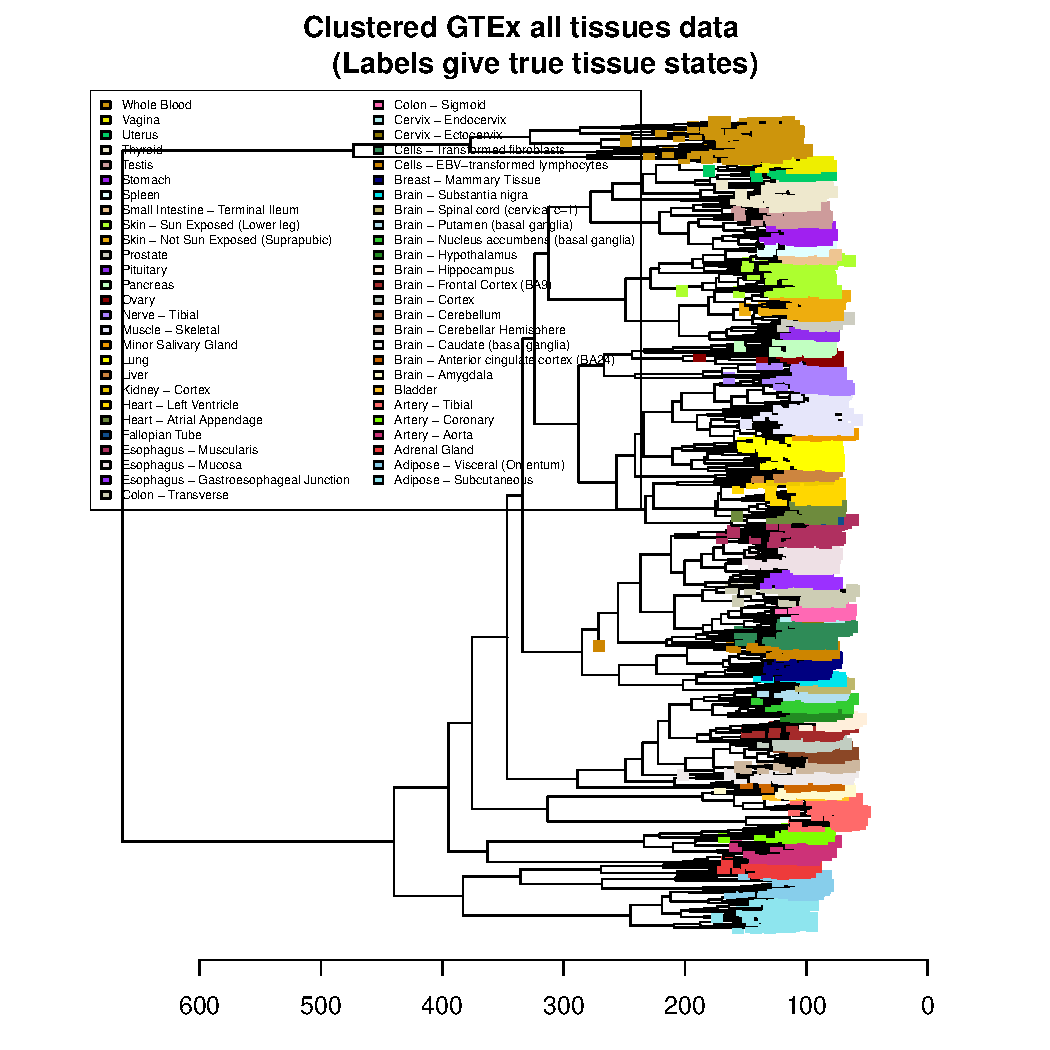
\includegraphics[height=6.3in, width=6in]{../../plots/dendextend_gtex.pdf}
\end{figure}

\end{document}

\clearpage
% adopt PLoS genetics environment settings
\documentclass[10pt,letterpaper]{article}
\usepackage[top=0.85in,left=2.75in,footskip=0.75in]{geometry}

% Template for PLoS
% Version 3.2 March 2016

% General commands for the entire paper
%
% Use Unicode characters when possible
\usepackage[utf8x]{inputenc}
% amsmath package, useful for mathematical formulas
\usepackage{amsmath}
%\usepackage{natbib}
% amssymb package, useful for mathematical symbols
\usepackage{amssymb}
\usepackage{booktabs}
\usepackage{xspace}
\usepackage{hyperref}
% graphicx package, useful for including eps and pdf graphics
% include graphics with the command \includegraphics
\usepackage{graphicx}

% Use adjustwidth environment to exceed column width (see example table in text)
\usepackage{changepage}

% textcomp package and marvosym package for additional characters
\usepackage{textcomp,marvosym}

% fixltx2e package for \textsubscript
\usepackage{fixltx2e}

% cite package, to clean up citations in the main text. Do not remove.
\usepackage{cite}
\usepackage{caption}
\usepackage{subcaption}
\usepackage{rotating}

\usepackage{color}

% Use doublespacing - comment out for single spacing
%\usepackage{setspace}
%\doublespacing

% Text layout
\topmargin 0.0cm
\oddsidemargin 0.5cm
\evensidemargin 0.5cm
\textwidth 16cm
\textheight 21cm

\setlength{\parskip}{1em}

% Bold the 'Figure #' in the caption and separate it with a period
% Captions will be left justified
\usepackage[labelfont=bf,labelsep=period,justification=raggedright]{caption}

% Use the PLoS provided bibtex style
\bibliographystyle{/Users/stephens/Dropbox/Documents/stylefiles/plos2009}

% Remove brackets from numbering in List of References
\makeatletter
\renewcommand{\@biblabel}[1]{\quad#1.}
\makeatother

% Use nameref to cite supporting information files (see Supporting Information section for more info)
\usepackage{nameref,hyperref}

% line numbers
\usepackage[right]{lineno}

% ligatures disabled
\usepackage{microtype}
\DisableLigatures[f]{encoding = *, family = * }

% Leave date blank
\date{}

\pagestyle{myheadings}
%% ** EDIT HERE **
\usepackage{enumerate}
\usepackage{multirow}
\usepackage{url}
\usepackage{xr} %for cross-referencing
%% ** EDIT HERE **
%% PLEASE INCLUDE ALL MACROS BELOW
\newtheorem{algorithm}{Algorithm}
\newtheorem{proposition}{Proposition}
\newtheorem{restateproposition}{Proposition}
\newtheorem{lemma}{Lemma}
\newtheorem{corollary}{Corollary}
\newtheorem{result}{Result}
\newtheorem{note}{Note}
\newtheorem{definition}{Definition}

\def\KL{\text{KL}}


% Text layout
\raggedright
\setlength{\parindent}{0.5cm}
\textwidth 5.25in
\textheight 8.75in

% Bold the 'Figure #' in the caption and separate it from the title/caption with a period
% Captions will be left justified
\usepackage[aboveskip=1pt,labelfont=bf,labelsep=period,justification=raggedright,singlelinecheck=off]{caption}
\renewcommand{\figurename}{Fig}

%------ bibliography
% Use the PLoS provided BiBTeX style
\bibliographystyle{plos2015}
% Remove brackets from numbering in List of References
\makeatletter
\renewcommand{\@biblabel}[1]{\quad#1.}
\makeatother


% Header and Footer with logo
\usepackage{lastpage,fancyhdr,graphicx}
\usepackage{epstopdf}
\pagestyle{myheadings}
\pagestyle{fancy}
\fancyhf{}
\setlength{\headheight}{27.023pt}
\lhead{\includegraphics[width=2.0in]{PLOS-submission.eps}}
\rfoot{\thepage/\pageref{LastPage}}
\renewcommand{\footrule}{\hrule height 2pt \vspace{2mm}}
\fancyheadoffset[L]{2.25in}
\fancyfootoffset[L]{2.25in}
\lfoot{\sf PLOS}

%% Include all macros below

\newcommand{\lorem}{{\bf LOREM}}
\newcommand{\ipsum}{{\bf IPSUM}}

%% END MACROS SECTION

%% Author's settings
\def\KL{\text{KL}}


% Text layout specific to Supplemental Materials
\topmargin 0.0cm
\oddsidemargin 0.5cm
\evensidemargin 0.5cm
\textwidth 16cm
\textheight 21cm

\setlength{\parskip}{1em}

\begin{document}

\paragraph*{S9 Fig.}

\label{figS9}
{\bf Comparison between GoM model and hierarchical in terms of power to separate samples from pairs of tissues.} A comparison of accuracy of GoM model vs hierarchical clustering.  Image plots to compare the GoM model with 4 different hierarchical clustering models on various transformations of the data. For each pair of tissues from the GTEx data we assessed whether or not each method (with $K=2$ clusters) separated the samples precisely according to their actual tissue of origin, with successful separation indicated by a filled square. Very clearly, the GoM model seems to be more successful in separating pairs of tissues compared to any of the hierarchical clustering approaches. In SubFig (a), hierarchical clustering was performed on log counts per million (cpm) data using Euclidean distance. In SubFig(b), the log cpm data data was mean and scale transformed for each gene and then the hierarchical clustering was performed on the transformed data using the Euclidean distance. In SubFig (d), the hierarchical clustering was  performed on counts data with the assumption the counts $c_{ng}$ for each gene have a variance  $\bar{c}_{g} + 1$, which we used to scale while computing distance matrix. In SubFig (e), we took the same scaled data as in SubFig(c), but we additionally performed mean and scale adjustments further so that all genes have expression of mean 0 and variance 1. In SubFig(c), GoM model is used to separate the tissues. Very clearly, GoM model seems to be performing better than any of the hierarchical methods.
\begin{figure}[ht]
\centering
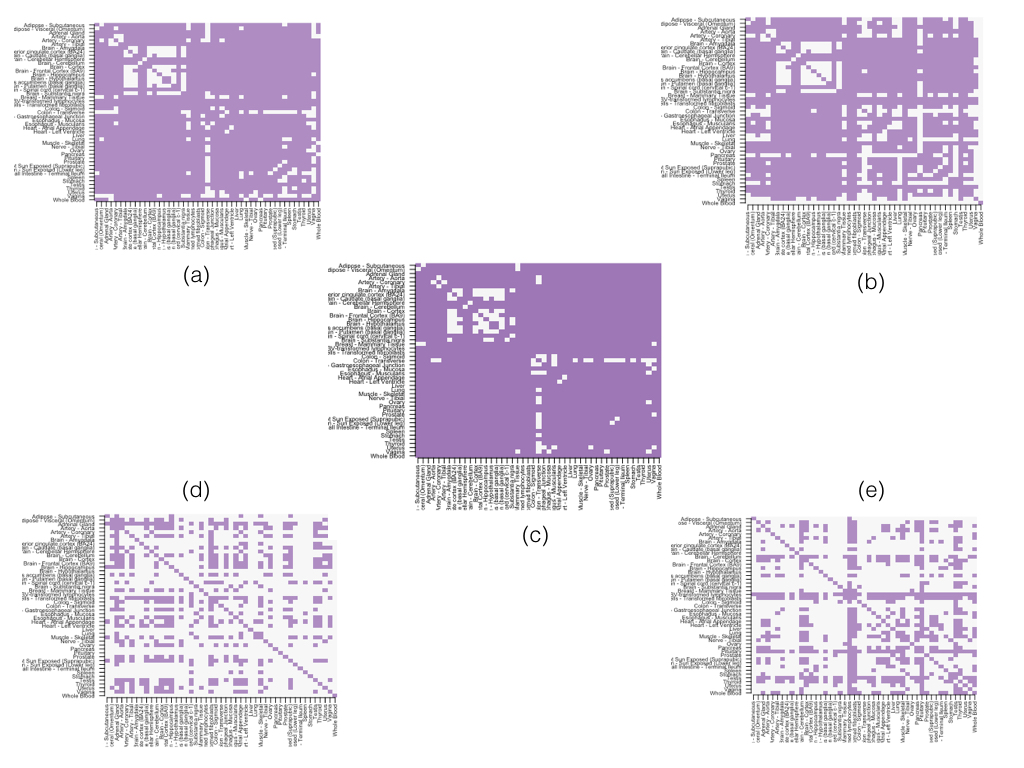
\includegraphics[height=6.3in, width=7in]{../../plots/gtex_hierarchical.jpeg}
\end{figure}

\end{document}

\clearpage

\section{Supplementary tables}
% adopt PLoS genetics environment settings
\documentclass[10pt,letterpaper]{article}
\usepackage[top=0.85in,left=2.75in,footskip=0.75in]{geometry}

% Template for PLoS
% Version 3.2 March 2016

% General commands for the entire paper
%
% Use Unicode characters when possible
\usepackage[utf8x]{inputenc}
% amsmath package, useful for mathematical formulas
\usepackage{amsmath}
%\usepackage{natbib}
% amssymb package, useful for mathematical symbols
\usepackage{amssymb}
\usepackage{booktabs}
\usepackage{xspace}
\usepackage{hyperref}
% graphicx package, useful for including eps and pdf graphics
% include graphics with the command \includegraphics
\usepackage{graphicx}

% Use adjustwidth environment to exceed column width (see example table in text)
\usepackage{changepage}

% textcomp package and marvosym package for additional characters
\usepackage{textcomp,marvosym}

% fixltx2e package for \textsubscript
\usepackage{fixltx2e}

% cite package, to clean up citations in the main text. Do not remove.
\usepackage{cite}
\usepackage{caption}
\usepackage{subcaption}
\usepackage{rotating}

\usepackage{color}

% Use doublespacing - comment out for single spacing
%\usepackage{setspace}
%\doublespacing

% Text layout
\topmargin 0.0cm
\oddsidemargin 0.5cm
\evensidemargin 0.5cm
\textwidth 16cm
\textheight 21cm

\setlength{\parskip}{1em}

% Bold the 'Figure #' in the caption and separate it with a period
% Captions will be left justified
\usepackage[labelfont=bf,labelsep=period,justification=raggedright]{caption}

% Use the PLoS provided bibtex style
\bibliographystyle{/Users/stephens/Dropbox/Documents/stylefiles/plos2009}

% Remove brackets from numbering in List of References
\makeatletter
\renewcommand{\@biblabel}[1]{\quad#1.}
\makeatother

% Use nameref to cite supporting information files (see Supporting Information section for more info)
\usepackage{nameref,hyperref}

% line numbers
\usepackage[right]{lineno}

% ligatures disabled
\usepackage{microtype}
\DisableLigatures[f]{encoding = *, family = * }

% Leave date blank
\date{}

\pagestyle{myheadings}
%% ** EDIT HERE **
\usepackage{enumerate}
\usepackage{multirow}
\usepackage{url}
\usepackage{xr} %for cross-referencing
%% ** EDIT HERE **
%% PLEASE INCLUDE ALL MACROS BELOW
\newtheorem{algorithm}{Algorithm}
\newtheorem{proposition}{Proposition}
\newtheorem{restateproposition}{Proposition}
\newtheorem{lemma}{Lemma}
\newtheorem{corollary}{Corollary}
\newtheorem{result}{Result}
\newtheorem{note}{Note}
\newtheorem{definition}{Definition}

\def\KL{\text{KL}}


% Text layout
\raggedright
\setlength{\parindent}{0.5cm}
\textwidth 5.25in
\textheight 8.75in

% Bold the 'Figure #' in the caption and separate it from the title/caption with a period
% Captions will be left justified
\usepackage[aboveskip=1pt,labelfont=bf,labelsep=period,justification=raggedright,singlelinecheck=off]{caption}
\renewcommand{\figurename}{Fig}

%------ bibliography
% Use the PLoS provided BiBTeX style
\bibliographystyle{plos2015}
% Remove brackets from numbering in List of References
\makeatletter
\renewcommand{\@biblabel}[1]{\quad#1.}
\makeatother


% Header and Footer with logo
\usepackage{lastpage,fancyhdr,graphicx}
\usepackage{epstopdf}
\pagestyle{myheadings}
\pagestyle{fancy}
\fancyhf{}
\setlength{\headheight}{27.023pt}
\lhead{\includegraphics[width=2.0in]{PLOS-submission.eps}}
\rfoot{\thepage/\pageref{LastPage}}
\renewcommand{\footrule}{\hrule height 2pt \vspace{2mm}}
\fancyheadoffset[L]{2.25in}
\fancyfootoffset[L]{2.25in}
\lfoot{\sf PLOS}

%% Include all macros below

\newcommand{\lorem}{{\bf LOREM}}
\newcommand{\ipsum}{{\bf IPSUM}}

%% END MACROS SECTION

%% Author's settings
\def\KL{\text{KL}}


% Text layout specific to Supplemental Materials
\topmargin 0.0cm
\oddsidemargin 0.5cm
\evensidemargin 0.5cm
\textwidth 16cm
\textheight 21cm

\setlength{\parskip}{1em}


\begin{document}

\paragraph*{S1 Table.}
\label{supptab1}
{\bf Cluster Annotations of GTEx V6 data with top driving gene summaries.}

\begin{table}[!hp]
\begin{adjustwidth}{-.5in}{0in}
\begin{tabular}{|p{0.6in}|p{0.6in}|p{1.3 in}|p{3.8in}|}
\hline
Cluster & Top Driving \qquad Genes & Gene names  & Gene Summary \\
\hline
\multirow{3}{4em}{\scriptsize{1. Royal purple} } &  \small{\textit{NEAT1}} & \scriptsize{nuclear paraspeckle assembly transcript 1} & \scriptsize{produces a long non-coding RNA (lncRNA) transcribed from the multiple endocrine neoplasia locus, regulates genes involved in cancer progression.}\\
				& \small{\textit{CCNL2}} & \scriptsize{cyclin L2} & \scriptsize{regulator of the pre-mRNA splicing process, as well as in inducing apoptosis by modulating the expression of apoptotic and antiapoptotic proteins.}\\
				& \small{\textit{SRSF5}} & \scriptsize{serine/arginine-rich splicing factor 5} & \scriptsize{encodes proteins of serine/arginine (SR)-rich family,  involved in mRNA export from the nucleus and in translation.}\\
\hline
 \multirow{3}{4em}{\scriptsize{2. Light purple} } & \small{\textit{SNAP25}}  & \scriptsize{synaptosomal-associated protein, 25kDa} & \scriptsize{this gene product is a presynaptic plasma membrane protein involved in the regulation of neurotransmitter release.} \\
 					&  \small{\textit{FBXL16}}  & \scriptsize{F-box and leucine-rich repeat protein 16} & \scriptsize{members of F-box protein family, which interact with SKP1 through the F box, and they interact with ubiquitination targets through other protein interaction domains.} \\
					&  \small{\textit{SLC17A7}}  & \scriptsize{neurochondrin} & \scriptsize{encodes proteins expressed in neuron-rich regions; associated with the membranes of synaptic vesicles and functions in glutamate transport.} \\
\hline
 \multirow{3}{4em}{\scriptsize{3. Red} } & \small{\textit{FABP4}}  & \scriptsize{fatty acid binding protein 4} & \scriptsize{ encodes the fatty acid binding protein found in adipocytes, takes part in fatty acid uptake, transport, and metabolism.} \\
 					&  \small{\textit{PLIN1}}  & \scriptsize{perilipin 1} & \scriptsize{protein encoded by this gene coats lipid storage droplets in adipocytes, thereby protecting them until they can be broken down by hormone-sensitive lipase.} \\
					&  \small{\textit{FASN}}  & \scriptsize{fatty acid synthase} & \scriptsize{catalyze the synthesis of palmitate from acetyl-CoA and malonyl-CoA, in the presence of NADPH, into long-chain saturated fatty acids.} \\
\hline
 \multirow{3}{4em}{\scriptsize{4. Salmon} } & \small{\textit{ACTG2}}  & \scriptsize{actin, gamma 2, smooth muscle, enteric} & \scriptsize{  involved in various types of cell motility and in the maintenance of the cytoskeleton.} \\
 					&  \small{\textit{MYH11}}  & \scriptsize{myosin, heavy chain 11, smooth muscle} & \scriptsize{protein encoded by this gene is a smooth muscle myosin belonging to the myosin heavy chain family, functions as a major contractile protein, converting chemical energy into mechanical energy through the hydrolysis of ATP.} \\
					&  \small{\textit{SYNM}}  & \scriptsize{synemin} & \scriptsize{protein has been found to form a linkage between desmin, which is a subunit of the IF network, and the extracellular matrix, and provides an important structural support in muscle.} \\
\hline
 \multirow{3}{4em}{\scriptsize{5. Denim} } & \small{\textit{RGS5}}  & \scriptsize{regulator of G-protein signaling 5} & \scriptsize{encodes a member of the regulators of G protein signaling (RGS) family, associated with retinal arterial macroaneurysm.} \\
 					&  \small{\textit{MFGE8}}  & \scriptsize{milk fat globule-EGF factor 8 protein} & \scriptsize{encodes a preproprotein that is proteolytically processed to form multiple protein products, been implicated in wound healing, autoimmune disease, and cancer} \\
					&  \small{\textit{ITGA8}}  & \scriptsize{synemin} & \scriptsize{Proteins generated mediate numerous cellular processes including cell adhesion, cytoskeletal rearrangement, and activation of cell signaling pathways.} \\			\hline
 \multirow{3}{4em}{\scriptsize{6. Light denim} } & \small{\textit{KRT10}}  & \scriptsize{keratin 10} & \scriptsize{encodes a member of the type I (acidic) cytokeratin family, mutations associated with epidermolytic hyperkeratosis.} \\
 					 &  \small{\textit{KRT1}} & \scriptsize{keratin 1, type II} & \scriptsize{specifically expressed in the spinous and granular layers of the epidermis with family member KRT10 and mutations in these genes have been associated with bullous congenital ichthyosiform erythroderma.} \\
					& \small{\textit{KRT2}} & \scriptsize{keratin 2, type II} & \scriptsize{expressed largely in the upper spinous layer of epidermal keratinocytes and mutations in this gene have been associated with bullous congenital ichthyosiform erythroderma.}\\
\hline
 \multirow{3}{4em}{\scriptsize{7. Orange} } & \small{\textit{NEB}} & \scriptsize{nebulin} & \scriptsize{encodes nebulin, a giant protein component of the cytoskeletal matrix that coexists with the thick and thin filaments within the sarcomeres of skeletal muscle, associated with recessive nemaline myopathy.}  \\
 					 & \small{\textit{MYH1}} & \scriptsize{myosin, heavy chain 1, skeletal muscle, adult }& \scriptsize{a major contractile protein which converts chemical energy into mechanical energy through the hydrolysis of ATP.} \\
					& \small{\textit{MYH2}} & \scriptsize{myosin, heavy chain 2, skeletal muscle, adult} & \scriptsize{encodes a member of the class II or conventional myosin heavy chains, and functions in skeletal muscle contraction.} \\
\hline
\end{tabular}
\end{adjustwidth}
\end{table}


\clearpage

\begin{table}[!hp]
\begin{adjustwidth}{-.5in}{0in}
\begin{tabular}{|p{0.6in}|p{0.6in}|p{1.3 in}|p{3.8in}|}
\hline
Cluster & Top Driving \qquad Genes & Gene namese  & Gene Summary \\
\hline
 \multirow{3}{4em}{\scriptsize{8. Light orange} } & \small{\textit{FN1}}  & \scriptsize{fibronectin 1} & \scriptsize{Fibronectin is involved in cell adhesion, embryogenesis, blood coagulation, host defense, and metastasis.}   \\
 					 & \small{\textit{COL1A1}} & \scriptsize{collagen, type I, alpha 1} & \scriptsize{Mutations in this gene associated with osteogenesis imperfecta types I-IV, Ehlers-Danlos syndrome type and Classical type, Caffey Disease}. \\
					      & \small{\textit{COL1A2}} & \scriptsize{collagen, type I, alpha 2} & \scriptsize{Mutations in this gene associated with osteogenesis imperfecta types I-IV, Ehlers-Danlos syndrome type and Classical type, Caffey Disease}. \\
\hline
 \multirow{3}{4em}{\scriptsize{9. Green} } & \small{\textit{MBP}} & \scriptsize{myelin basic protein} & \scriptsize{major constituent of the myelin sheath of oligodendrocytes and Schwann cells in the nervous system}    \\
 					 & \small{\textit{GFAP}} & \scriptsize{glial fibrillary acidic protein} & \scriptsize{encodes one of the major intermediate filament proteins of mature astrocytes, mutations casuses Alexander disease.} \\
					      & \small{\textit{CARNS1}} & \scriptsize{carnosine synthase 1} & \scriptsize{catalyzes the formation of carnosine and homocarnosine, which are found mainly in skeletal muscle and the central nervous system, respectively}. \\
\hline
 \multirow{3}{4em}{\scriptsize{10. Light green} } & \small{\textit{CYP17A1}} & \scriptsize{cytochrome P450 family 17 subfamily A member 1} & \scriptsize{encodes a member of the cytochrome P450 superfamily of enzymes, mutations in this gene are associated with isolated steroid-17 alpha-hydroxylase deficiency,20-lyase deficiency, pseudohermaphroditism, and adrenal hyperplasia.}    \\
 					 & \small{\textit{CYP11B1}} & \scriptsize{cytochrome P450 family 11 subfamily B member 1} & \scriptsize{The protein encoded by this gene plays a key role in the acute regulation of steroid hormone synthesis by enhancing the conversion of cholesterol into pregnenolone, associated with congenital lipoid adrenal hyperplasia.} \\
					      & \small{\textit{GKN1}} & \scriptsize{gastrokine 1} & \scriptsize{protein encoded by this gene is found to be down-regulated in human gastric cancer tissue as compared to normal gastric mucosa.}. \\
\hline
\multirow{3}{4em}{\scriptsize{11. Turquoise} } & \small{\textit{MPZ}} & \scriptsize{myelin protein zero} & \scriptsize{specifically expressed in Schwann cells of the peripheral nervous system and encodes a type I transmembrane glycoprotein that is a major structural protein of the peripheral myelin sheath, mutations  associated with autosomal dominant form of Charcot-Marie-Tooth disease type 1 and other polyneuropathies.}    \\
 					 & \small{\textit{APOD}} & \scriptsize{apolipoprotein D} & \scriptsize{encodes a component of high density lipoprotein that has no marked similarity to other apolipoprotein sequences, closely associated with lipoprotein metabolism.} \\
					      & \small{\textit{PMP22}} & \scriptsize{peripheral myelin protein 22} & \scriptsize{encodes an integral membrane protein that is a major component of myelin in the peripheral nervous system.}. \\
\hline
\multirow{3}{4em}{\scriptsize{12. Yellow} } & \small{\textit{IGHM}} & \scriptsize{immunoglobulin heavy constant mu} & \scriptsize{IgM antibodies play an important role in primary defense mechanisms, Diseases associated with IGHM include agammaglobulinemia 1 and immunodeficiency 23.}    \\
 					 & \small{\textit{IGHG1}} & \scriptsize{immunoglobulin heavy constant gamma 1 (G1m marker)} & \scriptsize{antigen binding functionality, diseases associated with IGHG1 include heavy chain deposition disease and chronic lymphocytic leukemia.} \\
					      & \small{\textit{IGHG2}} & \scriptsize{immunoglobulin heavy constant gamma 2 (G2m marker)} & \scriptsize{antigen binding gene, diseases associated with IGHG2 include c2 deficiency}. \\
\hline
\multirow{3}{4em}{\scriptsize{13. Sky blue} } & \small{\textit{TG}} & \scriptsize{thyroglobulin} & \scriptsize{thyroglobulin produced predominantly in thyroid gland, synthesizes thyroxine and triiodothyronine, associated with Graves disease and Hashimotot thyroiditis.} \\
 					 &  \small{\textit{PRL}} & \scriptsize{prolactin 2} & \scriptsize{encodes the anterior pituitary hormone prolactin. This secreted hormone is a growth regulator for many tissues, including cells of the immune system.}  \\
					      & \small{\textit{PRM2}} & \scriptsize{protamine 2} & \scriptsize{Protamines are the major DNA-binding proteins in the nucleus of sperm}. \\
\hline
\multirow{3}{4em}{\scriptsize{14. Light pink} } & \small{\textit{NPPA}} & \scriptsize{natriuretic peptide A} & \scriptsize{protein encoded by this gene belongs to the natriuretic peptide family, controls extracellular fluid volume and electrolyte homeostasis, mutations Mutations associated with atrial fibrillation familial type 6.} \\
 					 &  \small{\textit{MYH6}} & \scriptsize{myosin, heavy chain 6, cardiac muscle, alpha} & \scriptsize{encodes the alpha heavy chain subunit of cardiac myosin,  mutations cause familial hypertrophic cardiomyopathy and atrial septal defect 3}  \\
					      & \small{\textit{TNNT2}} & \scriptsize{protamine 2} & \scriptsize{protein encoded by this gene is the tropomyosin-binding subunit of the troponin complex, mutations in this gene have been associated with familial hypertrophic cardiomyopathy as well as with dilated cardiomyopathy}. \\
\hline
\end{tabular}
\end{adjustwidth}
\end{table}


\clearpage
\begin{table}[!hp]
\begin{adjustwidth}{-.5in}{0in}
\begin{tabular}{|p{0.6in}|p{0.6in}|p{1.3 in}|p{3.8in}|}
\hline
Cluster & Top Driving \qquad Genes & Gene namese  & Gene Summary \\
\hline
\multirow{3}{4em}{\scriptsize{15. Light gray} } &  \small{\textit{KRT13}} & \scriptsize{keratin 13, type I} & \scriptsize{protein encoded by this gene is a member of the keratin gene family, associated with the autosomal dominant disorder White Sponge Nevus.}\\
 					 &  \small{\textit{KRT4}} & \scriptsize{keratin 4, type II} & \scriptsize{protein encoded by this gene is a member of the keratin gene family, associated with White Sponge Nevus, characterized by oral, esophageal, and anal leukoplakia.} \\
					      &  \small{\textit{CRNN}} & \scriptsize{cornulin} & \scriptsize{may play a role in the mucosal/epithelial immune response and epidermal differentiation. } \\
\hline
\multirow{3}{4em}{\scriptsize{16. Gray} } & \small{\textit{SFTPB}} & \scriptsize{surfactant protein B} & \scriptsize {an amphipathic surfactant protein essential for lung function and homeostasis after birth, muttaions cause pulmonary alveolar proteinosis, fatal respiratory distress in the neonatal period.} \\
 					    & \small{\textit{SFTPA2}} & \scriptsize{surfactant protein A2} & \scriptsize{Mutations in this gene and a highly similar gene located nearby, which affect the highly conserved carbohydrate recognition domain, are associated with idiopathic pulmonary fibrosis.} \\
					    & \small{\textit{SFTPA1}} & \scriptsize{surfactant protein A1} &  \scriptsize{encodes a lung surfactant protein that is a member of C-type lectins called collectins, associated with idiopathic pulmonary fibrosis.} \\
\hline
\multirow{3}{4em}{\scriptsize{17. Brown} } & \small{\textit{CSF3R}} & \scriptsize{colony stimulating factor 3 receptor} & \scriptsize {protein encoded by this gene is the receptor for colony stimulating factor 3, a cytokine that controls the production, differentiation, and function of granulocytes, mutations a cause of Kostmann syndrome} \\
 					    & \small{\textit{MMP25}} & \scriptsize{matrix metallopeptidase 25} & \scriptsize{proteins are involved in the breakdown of extracellular matrix in normal physiological processes, such as embryonic development, reproduction, and tissue remodeling, as well as in disease processes, such as arthritis and metastasis.} \\
					    & \small{\textit{IL1R2}} & \scriptsize{interleukin 1 receptor type 2} &  \scriptsize{protein encoded by this gene is a cytokine receptor that belongs to the interleukin 1 receptor family.} \\
\hline
\multirow{3}{4em}{\scriptsize{18. Purple} } &  \small{\textit{PRSS1}} & \scriptsize{protease, serine 1} & \scriptsize{secreted by pancreas, associated with pancreatitis}\\
 					      &  \small{\textit{CPA1}} & \scriptsize{carboxypeptidase A1} & \scriptsize{secreted by pancreas, linked to pancreatitis and pancreatic cancer} \\
					      &  \small{\textit{PNLIP}} & \scriptsize{pancreatic lipase} & \scriptsize{encodes a carboxyl esterase that hydrolyzes insoluble, emulsified triglycerides, and is essential for the efficient digestion of dietary fats. This gene is expressed specifically in the pancreas.}\\
\hline
\multirow{3}{4em}{\scriptsize{19. Pink} } & \small{\textit{HBB}} & \scriptsize{hemoglobin, beta} & \scriptsize{mutant beta globin causes sickle cell anemia, absence of beta chain/ reduction in beta globin leads to thalassemia.}\\
 					      & \small{\textit{HBA2}} & \scriptsize{hemoglobin, alpha 2} & \scriptsize{deletion of alpha genes may lead to alpha thalassemia.}  \\
					      & \small{\textit{HBA1}} & \scriptsize{hemoglobin, alpha 1} & \scriptsize{deletion of alpha genes may lead to alpha thalassemia.}  \\
\hline
\multirow{3}{4em}{\scriptsize{20. Dark gray} } &  \small{\textit{ALB}} & \scriptsize{albumin} & \scriptsize{functions primarily as a carrier protein for steroids, fatty acids, and thyroid hormones and plays a role in stabilizing extracellular fluid volume.} \\
					      &  \small{\textit{HP}} & \scriptsize{haptoglobin} & \scriptsize{encodes a preproprotein, which subsequently  produces haptoglobin, linked to diabetic nephropathy, Crohn's disease, inflammatory disease behavior and reduced incidence of Plasmodium falciparum malaria.}\\
					      & \small{\textit{FGB}} & \scriptsize{fibrinogen beta chain} & \scriptsize{protein encoded by this gene is the beta component of fibrinogen, mutations may lead to several disorders, including afibrinogenemia, dysfibrinogenemia, hypodysfibrinogenemia etc.}  \\
\hline
\end{tabular}
\end{adjustwidth}
\end{table}

\end{document}

\clearpage
\documentclass[10pt,letterpaper]{article}
\usepackage[top=0.85in,left=2.75in,footskip=0.75in]{geometry}

% Template for PLoS
% Version 3.2 March 2016

% General commands for the entire paper
%
% Use Unicode characters when possible
\usepackage[utf8x]{inputenc}
% amsmath package, useful for mathematical formulas
\usepackage{amsmath}
%\usepackage{natbib}
% amssymb package, useful for mathematical symbols
\usepackage{amssymb}
\usepackage{booktabs}
\usepackage{xspace}
\usepackage{hyperref}
% graphicx package, useful for including eps and pdf graphics
% include graphics with the command \includegraphics
\usepackage{graphicx}

% Use adjustwidth environment to exceed column width (see example table in text)
\usepackage{changepage}

% textcomp package and marvosym package for additional characters
\usepackage{textcomp,marvosym}

% fixltx2e package for \textsubscript
\usepackage{fixltx2e}

% cite package, to clean up citations in the main text. Do not remove.
\usepackage{cite}
\usepackage{caption}
\usepackage{subcaption}
\usepackage{rotating}

\usepackage{color}

% Use doublespacing - comment out for single spacing
%\usepackage{setspace}
%\doublespacing

% Text layout
\topmargin 0.0cm
\oddsidemargin 0.5cm
\evensidemargin 0.5cm
\textwidth 16cm
\textheight 21cm

\setlength{\parskip}{1em}

% Bold the 'Figure #' in the caption and separate it with a period
% Captions will be left justified
\usepackage[labelfont=bf,labelsep=period,justification=raggedright]{caption}

% Use the PLoS provided bibtex style
\bibliographystyle{/Users/stephens/Dropbox/Documents/stylefiles/plos2009}

% Remove brackets from numbering in List of References
\makeatletter
\renewcommand{\@biblabel}[1]{\quad#1.}
\makeatother

% Use nameref to cite supporting information files (see Supporting Information section for more info)
\usepackage{nameref,hyperref}

% line numbers
\usepackage[right]{lineno}

% ligatures disabled
\usepackage{microtype}
\DisableLigatures[f]{encoding = *, family = * }

% Leave date blank
\date{}

\pagestyle{myheadings}
%% ** EDIT HERE **
\usepackage{enumerate}
\usepackage{multirow}
\usepackage{url}
\usepackage{xr} %for cross-referencing
%% ** EDIT HERE **
%% PLEASE INCLUDE ALL MACROS BELOW
\newtheorem{algorithm}{Algorithm}
\newtheorem{proposition}{Proposition}
\newtheorem{restateproposition}{Proposition}
\newtheorem{lemma}{Lemma}
\newtheorem{corollary}{Corollary}
\newtheorem{result}{Result}
\newtheorem{note}{Note}
\newtheorem{definition}{Definition}

\def\KL{\text{KL}}


% Text layout
\raggedright
\setlength{\parindent}{0.5cm}
\textwidth 5.25in
\textheight 8.75in

% Bold the 'Figure #' in the caption and separate it from the title/caption with a period
% Captions will be left justified
\usepackage[aboveskip=1pt,labelfont=bf,labelsep=period,justification=raggedright,singlelinecheck=off]{caption}
\renewcommand{\figurename}{Fig}

%------ bibliography
% Use the PLoS provided BiBTeX style
\bibliographystyle{plos2015}
% Remove brackets from numbering in List of References
\makeatletter
\renewcommand{\@biblabel}[1]{\quad#1.}
\makeatother


% Header and Footer with logo
\usepackage{lastpage,fancyhdr,graphicx}
\usepackage{epstopdf}
\pagestyle{myheadings}
\pagestyle{fancy}
\fancyhf{}
\setlength{\headheight}{27.023pt}
\lhead{\includegraphics[width=2.0in]{PLOS-submission.eps}}
\rfoot{\thepage/\pageref{LastPage}}
\renewcommand{\footrule}{\hrule height 2pt \vspace{2mm}}
\fancyheadoffset[L]{2.25in}
\fancyfootoffset[L]{2.25in}
\lfoot{\sf PLOS}

%% Include all macros below

\newcommand{\lorem}{{\bf LOREM}}
\newcommand{\ipsum}{{\bf IPSUM}}

%% END MACROS SECTION

%% Author's settings
\def\KL{\text{KL}}


\begin{document}

\paragraph*{S2 Table.}
\label{supptab2}
{\bf Cluster Annotations of GTEx V6 Brain data with top driving gene summaries.}

\begin{table}[!hp]
\begin{adjustwidth}{-.5in}{0in}
\begin{tabular}{|p{0.7in}|p{0.7in}|p{1.4in}|p{3.6in}|}
\hline
Cluster & Top Driving \qquad Genes & Gene names & Gene Summary \\
\hline
 \multirow{3}{4em}{\small{1, Royal blue}}  &  \small{\textit{CLU}} &  \footnotesize{clusterin} & \scriptsize{protein encoded by this gene is a secreted chaperone that can under some stress conditions also be found in the cell cytosol, also involved in cell death, tumor progression, and neurodegenerative disorders.} \\
 					      & \small{\textit{OXT}} &  \footnotesize{oxytocin/neurophysin I prepropeptide} & \scriptsize{encodes a precursor protein that is processed to produce oxytocin and neurophysin I, involved in contraction of  smooth muscle during parturition and lactation, cognition, tolerance, adaptation and complex sexual and maternal behaviour.} \\
					      & \small{\textit{GLUL}} & \footnotesize{glutamate-ammonia ligase} & \scriptsize{catalyzes the synthesis of glutamine from glutamate and ammonia in an ATP-dependent reaction,  associated with congenital glutamine deficiency, and overexpression of this gene was observed in some primary liver cancer samples.} \\
\hline
 \multirow{3}{4em}{\small{2, Turquoise}}  & \small{\textit{ENC1}} & \footnotesize{ectodermal-neural cortex 1} & \scriptsize{plays a role in the oxidative stress response as a regulator of the transcription factor Nrf2, may play role in malignant transformation.} \\
 							&  \small{\textit{NCALD}} & \footnotesize{neurocalcin delta} & \scriptsize{ encodes a member of the neuronal calcium sensor (NCS), a regulator of G protein-coupled receptor signal transduction.}   \\
 					      & \small{\textit{YWHAH}} &  \footnotesize{tyrosine 3-monooxygenase/tryptophan 5-monooxygenase activation protein eta} & \scriptsize{mediate signal transduction by binding to phosphoserine-containing proteins, associated with early-onset schizophrenia and psychotic bipolar disorder.} \\
\hline
 \multirow{3}{4em}{\small{3, Lime green}} & \small{\textit{PKD1}} & \footnotesize{polycystin 1, transient receptor potential channel interacting} & \scriptsize{functions as a regulator of calcium permeable cation channels and intracellular calcium homoeostasis. It is also involved in cell-cell/matrix interactions and may modulate G-protein-coupled signal-transduction pathways.}\\
 					    & \small{\textit{CBLN3}} & \footnotesize{cerebellin 3 precursor} & \scriptsize{ contain a cerebellin motif and C-terminal C1q signature domain that mediates trimeric assembly of atypical collagen complexes} \\
					    &  \small{\textit{CHGB}} &  \footnotesize{chromogranin B} & \scriptsize{ encodes a tyrosine-sulfated secretory protein abundant in peptidergic endocrine cells and neurons. This protein may serve as a precursor for regulatory peptides.} \\
 \hline
  \multirow{3}{4em}{\small{4, Red}} & \small{\textit{PPP1R1B}} & \footnotesize{protein phosphatase 1 regulatory inhibitor sub-
unit 1B} & \scriptsize{encodes a bifunctional signal transduction molecule, may serve as a therapeutic target for neurologic and psychiatric disorders.}\\
 					    & \small{\textit{RGS14}} & \footnotesize{regulator of G-protein signaling 14} & \scriptsize{ attenuates the signaling activity of G-proteins, increases the rate of conversion of the GTP to GDP.} \\
					    &  \small{\textit{NCDN}} &  \footnotesize{neurochondrin} & \scriptsize{ encodes a leucine-rich cytoplasmic protein, essential for spatial learning processes.} \\
 \hline
 \multirow{3}{4em}{\small{5, Yellow orange}} & \small{\textit{MBP}} & \footnotesize{myelin basic protein} & \scriptsize{protein encoded is a major constituent of the myelin sheath of oligodendrocytes and Schwann cells in the nervous system.} \\
 					    & \small{\textit{GFAP}} & \footnotesize{glial fibrillary acidic protein} & \scriptsize{ encodes major intermediate filament proteins of mature astrocytes, a marker to distinguish astrocytes during development, mutations in this gene cause Alexander disease, a rare disorder of astrocytes in central nervous system.} \\
					    & \small{\textit{TF}}  & \footnotesize{transferrin}  & \scriptsize{transport iron from the intestine, reticuloendothelial system, and liver parenchymal cells to all proliferating cells in the body, involved in the removal of certain organic matter and allergens from serum.}\\
\hline
 \multirow{3}{4em}{\small{6, Yellow}} & \small{\textit{IQGAP1}} & \footnotesize{IQ motif containing GTPase activating protein 1} & \scriptsize{interacts with components of the cytoskeleton, with cell adhesion molecules, and with several signaling molecules to regulate cell morphology and motility.} \\
 					    & \small{\textit{A2M}} & \footnotesize{alpha-2-macroglobulin} & \scriptsize{ inhibits many proteases, including trypsin, thrombin and collagenase. A2M is implicated in Alzheimer disease (AD) due to its ability to mediate the clearance and degradation of A-beta, the major component of beta-amyloid deposits.} \\
					    & \small{\textit{C3}}  & \footnotesize{complement component 3}  & \scriptsize{plays a central role in the activation of complement system, associated with atypical hemolytic uremic syndrome and age-related macular degeneration in human patients.}\\
\hline
\end{tabular}
\end{adjustwidth}
\end{table}

\end{document}

\clearpage
\documentclass[10pt,letterpaper]{article}
\usepackage[top=0.85in,left=2.75in,footskip=0.75in]{geometry}

% Template for PLoS
% Version 3.2 March 2016

% General commands for the entire paper
%
% Use Unicode characters when possible
\usepackage[utf8x]{inputenc}
% amsmath package, useful for mathematical formulas
\usepackage{amsmath}
%\usepackage{natbib}
% amssymb package, useful for mathematical symbols
\usepackage{amssymb}
\usepackage{booktabs}
\usepackage{xspace}
\usepackage{hyperref}
% graphicx package, useful for including eps and pdf graphics
% include graphics with the command \includegraphics
\usepackage{graphicx}

% Use adjustwidth environment to exceed column width (see example table in text)
\usepackage{changepage}

% textcomp package and marvosym package for additional characters
\usepackage{textcomp,marvosym}

% fixltx2e package for \textsubscript
\usepackage{fixltx2e}

% cite package, to clean up citations in the main text. Do not remove.
\usepackage{cite}
\usepackage{caption}
\usepackage{subcaption}
\usepackage{rotating}

\usepackage{color}

% Use doublespacing - comment out for single spacing
%\usepackage{setspace}
%\doublespacing

% Text layout
\topmargin 0.0cm
\oddsidemargin 0.5cm
\evensidemargin 0.5cm
\textwidth 16cm
\textheight 21cm

\setlength{\parskip}{1em}

% Bold the 'Figure #' in the caption and separate it with a period
% Captions will be left justified
\usepackage[labelfont=bf,labelsep=period,justification=raggedright]{caption}

% Use the PLoS provided bibtex style
\bibliographystyle{/Users/stephens/Dropbox/Documents/stylefiles/plos2009}

% Remove brackets from numbering in List of References
\makeatletter
\renewcommand{\@biblabel}[1]{\quad#1.}
\makeatother

% Use nameref to cite supporting information files (see Supporting Information section for more info)
\usepackage{nameref,hyperref}

% line numbers
\usepackage[right]{lineno}

% ligatures disabled
\usepackage{microtype}
\DisableLigatures[f]{encoding = *, family = * }

% Leave date blank
\date{}

\pagestyle{myheadings}
%% ** EDIT HERE **
\usepackage{enumerate}
\usepackage{multirow}
\usepackage{url}
\usepackage{xr} %for cross-referencing
%% ** EDIT HERE **
%% PLEASE INCLUDE ALL MACROS BELOW
\newtheorem{algorithm}{Algorithm}
\newtheorem{proposition}{Proposition}
\newtheorem{restateproposition}{Proposition}
\newtheorem{lemma}{Lemma}
\newtheorem{corollary}{Corollary}
\newtheorem{result}{Result}
\newtheorem{note}{Note}
\newtheorem{definition}{Definition}

\def\KL{\text{KL}}


% Text layout
\raggedright
\setlength{\parindent}{0.5cm}
\textwidth 5.25in
\textheight 8.75in

% Bold the 'Figure #' in the caption and separate it from the title/caption with a period
% Captions will be left justified
\usepackage[aboveskip=1pt,labelfont=bf,labelsep=period,justification=raggedright,singlelinecheck=off]{caption}
\renewcommand{\figurename}{Fig}

%------ bibliography
% Use the PLoS provided BiBTeX style
\bibliographystyle{plos2015}
% Remove brackets from numbering in List of References
\makeatletter
\renewcommand{\@biblabel}[1]{\quad#1.}
\makeatother


% Header and Footer with logo
\usepackage{lastpage,fancyhdr,graphicx}
\usepackage{epstopdf}
\pagestyle{myheadings}
\pagestyle{fancy}
\fancyhf{}
\setlength{\headheight}{27.023pt}
\lhead{\includegraphics[width=2.0in]{PLOS-submission.eps}}
\rfoot{\thepage/\pageref{LastPage}}
\renewcommand{\footrule}{\hrule height 2pt \vspace{2mm}}
\fancyheadoffset[L]{2.25in}
\fancyfootoffset[L]{2.25in}
\lfoot{\sf PLOS}

%% Include all macros below

\newcommand{\lorem}{{\bf LOREM}}
\newcommand{\ipsum}{{\bf IPSUM}}

%% END MACROS SECTION

%% Author's settings
\def\KL{\text{KL}}


\begin{document}

\paragraph*{S3 Table.}
\label{supptab3}
{\bf Cluster Annotations of Deng data with top driving genes.}

\begin{table}[!hp]
\begin{adjustwidth}{-.5in}{0in}
\begin{tabular}{|c|c|p{1.5in}|p{4in}|}
  \hline
  & GO ID & GO Term  & Top Driving Genes \\
  \hline
1 & GO:0007276 & gamete generation & \footnotesize{BCL2L10; GDF9; NOBOX; PABPC1L; RGS2; CREB3L4; RNF114; BMP15; PTTG1; TDRD12; WEE2; SPIN1; DAZL} \\
  2 & GO:0007292 & female gamete generation & \footnotesize{GDF9; BCL2L10; PABPC1L; BMP15; WEE2; DAZL; NOBOX} \\
  3 & GO:0048609 & multicellular organismal reproductive process & \footnotesize{GDF9; NOBOX; PABPC1L; BCL2L10; BMP15; CREB3L4; TGFB2; RNF114; RGS2; PTTG1; TDRD12; WEE2; SPIN1; DAZL} \\
  4 & GO:0032504 & multicellular organism reproduction & \footnotesize{GDF9; NOBOX; PABPC1L; BCL2L10; BMP15; CREB3L4; TGFB2; RNF114; RGS2; PTTG1; TDRD12; WEE2; SPIN1; DAZL}\\
  5 & GO:0019953 & sexual reproduction & \footnotesize{BCL2L10; GDF9; NOBOX; PABPC1L; RGS2; CREB3L4; RNF114; BMP15; PTTG1; TDRD12; WEE2; SPIN1; DAZL} \\
  6 & GO:0044702 & single organism reproductive process & \footnotesize{GDF9; NOBOX; PABPC1L; BCL2L10; BMP15; CREB3L4; TGFB2; CASP8; RNF114; RGS2; PTTG1; TDRD12; WEE2; SPIN1; DAZL} \\
  7 & GO:0048477 & oogenesis & \footnotesize{WEE2; GDF9; NOBOX; PABPC1L; DAZL} \\
  8 & GO:0044703 & multi-organism reproductive process & \footnotesize{BCL2L10; GDF9; NOBOX; PABPC1L; RGS2; CREB3L4; RNF114; BMP15; PTTG1; TDRD12; WEE2; SPIN1; DAZL} \\
  9 & GO:0048599 & oocyte development  & \footnotesize{WEE2; GDF9; PABPC1L; DAZL} \\
  10 & GO:0009994 & oocyte differentiation & \footnotesize{WEE2; GDF9; PABPC1L; DAZL} \\
  11 & GO:0051321 & meiotic cell cycle & \footnotesize{H1FOO; WEE2; TDRD12; SPIN1; PTTG1; DAZL} \\
  12 & GO:0001556 & oocyte maturation & \footnotesize{WEE2; PABPC1L; DAZL} \\
  13 & GO:0006306 & DNA methylation & \footnotesize{TDRD12; H1FOO; TET3; ZFP57} \\
  14 & GO:0051302 & regulation of cell division & \footnotesize{TGFB2; PTTG1; TXNIP; WEE2; CHEK1; DAZL} \\
  15 & GO:0060255 & regulation of macromolecule metabolic process & \footnotesize{TGFB2; NOBOX; BPGM; UBE2D3; NFYA; CASP8; BMP15; TXNIP; TDRD12; GDF9; BCL2L10} \\
 \hline
\end{tabular}
\end{adjustwidth}
\end{table}


\paragraph*{S3 Table continued.}
{\bf Deng et al (2014) Cluster 2 (magenta) top GO annotations.}

\begin{table}[!hp]
\begin{adjustwidth}{-.5in}{0in}
\begin{tabular}{|c|c|p{1.5in}|p{4in}|}
  \hline
 & GO ID & GO Term  & Top Driving Genes \\
  \hline
1 & GO:0016604 & nuclear body  & \footnotesize{YTHDC1; RBM8A; CDK12; PSME4; PPP1R8; HIPK1; TOPORS} \\
  2 & GO:0005814 & centriole  & \footnotesize{SFI1; PLK2; ROCK1; TOPORS} \\
  3 & GO:0044450 & microtubule organizing center part  & \footnotesize{SFI1; PLK2; ROCK1; TOPORS} \\
   \hline
\end{tabular}
 \end{adjustwidth}
  \end{table}


\clearpage
\paragraph*{S3 Table continued.}
{\bf Deng et al (2014) Cluster 3 (yellow) top GO annotations.}

\begin{table}[!hp]
\begin{adjustwidth}{-.5in}{0in}
\begin{tabular}{|c|c|p{1.5in}|p{4in}|}
  \hline
 & GO ID & GO Term  & Top Driving Genes \\
  \hline
1 & GO:0044428 & nuclear part  & \footnotesize{MAD2L2; SMARCC1; PPRC1; SLU7; NFYB; TOR1B; MIOS; NR1H3; POLR3K} \\
  2 & GO:0031981 & nuclear lumen & \footnotesize{MAD2L2; SMARCC1; PPRC1; SLU7; NFYB; POLR1E; MIOS; POLR3K; XPO1}\\
  3 & GO:0070013 & intracellular organelle lumen & \footnotesize{MAD2L2; SMARCC1; PPRC1; SLU7; NFYB; POLR1E; MIOS; POLR3K; XPO1; DNTTIP2; ZBTB10; ZBTB17} \\
  4 & GO:0043233 & organelle lumen & \footnotesize{MAD2L2; SMARCC1; PPRC1; SLU7; NFYB; POLR1E; MIOS; POLR3K; XPO1} \\
  5 & GO:0005730 & nucleolus & \footnotesize{XPO1; DNTTIP2; ESF1; WDR43; ZDHHC7; HEATR1; POLR1E; DDX24; POLR3K} \\
  6 & GO:0005634 & nucleus & \footnotesize{MAD2L2; SMARCC1; PPRC1; SLU7; NFYB; TOR1B; MIOS; NR1H3; EIF5B; POLR3K} \\
  7 & GO:0044446 & intracellular organelle part & \footnotesize{MAD2L2; PTDSS2; SMARCC1; KLHL21; TOR1B; PPRC1; SLU7; NFYB; SLC25A36; ECE2} \\
  8 & GO:0005654 & nucleoplasm & \footnotesize{MAD2L2; SMARCC1; PPRC1; SLU7; NFYB; POLR1E; MIOS; POLR3K; XPO1; ZBTB10; ZBTB17} \\
  9 & GO:0003723 & RNA binding & \footnotesize{PPRC1; EIF5B; XPO1; DNTTIP2; WDR43; DDX10; EIF3C; BCLAF1; EBNA1BP2; RARS}\\
  10 & GO:0003676 & nucleic acid binding & \footnotesize{SMARCC1; PPRC1; SLU7; NFYB; POLR1E; EIF5B; POLR3K; XPO1; DNTTIP2} \\
  11 & GO:0043231 & intracellular membrane-bounded organelle &  \footnotesize{MAD2L2; PTDSS2; SMARCC1; TOR1B; PPRC1; SLU7; NFYB; ESF1; ECE2; LMAN1L} \\
  12 & GO:0043229 & intracellular organelle & \footnotesize{MAD2L2; PTDSS2; SMARCC1; KLHL21; TOR1B; PPRC1; ARRDC1; SLU7; NFYB; ESF1; ECE2} \\
  13 & GO:0005874 & microtubule & \footnotesize{WDR43; KLHL21; HAUS6; CENPE; TEKT2; RACGAP1; WDR81; BCL2L11; KIF20B} \\
  14 & GO:0044822 & poly(A) RNA binding & \footnotesize{WDR43; DNTTIP2; ESF1; NXF1; DDX10; HEATR1; EIF3C} \\
  15 & GO:0044424 & intracellular part & \footnotesize{MAD2L2; PTDSS2; SMARCC1; KLHL21; TOR1B; PPRC1; SNAPC4; POLR3K; ARRDC1; SLU7; NFYB; ESF1; WDR43; ECE2; LMAN1L} \\
%  16 & GO:0043228 & non-membrane-bounded organelle & c & 3207 & MAD2L2; SMARCC1; KLHL21; WDR81; POLR3K; XPO1; DNTTIP2; WDR43; BCL2L11; YPEL2; HAUS6; TEKT2; BCLAF1; NF2; URB2; NR1H3; ESF1; HEATR1; CENPE; EIF4E; USP33; EBNA1BP2; PAFAH1B2; NASP; ZDHHC7; DDX24; TRAIP; RACGAP1; WDR36; POLRMT; ATXN7; KIF20B; KDM5A; POLR1E \\
%  17 & GO:0043232 & intracellular non-membrane-bounded organelle & c & 3207 & MAD2L2; SMARCC1; KLHL21; WDR81; POLR3K; XPO1; DNTTIP2; WDR43; BCL2L11; YPEL2; HAUS6; TEKT2; BCLAF1; NF2; URB2; NR1H3; ESF1; HEATR1; CENPE; EIF4E; USP33; EBNA1BP2; PAFAH1B2; NASP; ZDHHC7; DDX24; TRAIP; RACGAP1; WDR36; POLRMT; ATXN7; KIF20B; KDM5A; POLR1E \\
%  18 & GO:0051233 & spindle midzone & c &  23 & RACGAP1; CENPE; KIF20B \\
%  19 & GO:0003847 & 1-alkyl-2-acetylglycerophosphocholine esterase activity & m &   5 & ASPG; PAFAH1B2 \\
%  20 & GO:1990023 & mitotic spindle midzone & c &   5 & CENPE; KIF20B \\
%  21 & GO:0008017 & microtubule binding & m & 169 & WDR43; BCL2L11; RACGAP1; CENPE; WDR81; KIF20B \\
%  22 & GO:0071014 & post-mRNA release spliceosomal complex & c &   6 & CRNKL1; TFIP11 \\
%  23 & GO:1901363 & heterocyclic compound binding & m & 4675 & SMARCC1; PPRC1; POLR3K; TFIP11; NFYB; TOR1B; EIF5B; CHKA; XPO1; DNTTIP2; ZBTB10; ZBTB17; DDX10; EIF3C; BCLAF1; CRNKL1; RARS; ITPKC; RANBP2; ESF1; NXF1; HEATR1; CENPE; SNUPN; PRKCD; SPIC; WDR43; SNAPC4; EIF4E; EBNA1BP2; UBR5; THAP4; SOS1; DDX24; PFKFB3; SLU7; GEMIN5; WDR36; POLRMT; NR1H3; KIF20B; KDM5A; POLR1E \\
%  24 & GO:0043227 & membrane-bounded organelle & c & 9724 & MAD2L2; PTDSS2; SMARCC1; TOR1B; PPRC1; SNAPC4; SLU7; NFYB; ESF1; ECE2; LMAN1L; MIOS; NR1H3; EIF5B; POLR3K; XPO1; DNTTIP2; ZBTB10; ZBTB17; NOB1; TFIP11; HAUS6; TEKT2; BCLAF1; CRNKL1; RARS; SLC25A36; NF2; CTNNBL1; URB2; MGEA5; RANBP2; POLR1E; ITPKC; SNUPN; CTSL; NXF1; HEATR1; CENPE; CTSC; NPC1L1; ATP1B3; RTN2; PRKCD; SPIC; TNIP1; LAMP2; GFPT1; EIF4E; BCL2L11; USP33; EBNA1BP2; UBR5; PAFAH1B2; GINS3; NASP; WDR43; ZDHHC7; DDX24; RACGAP1; PFKFB3; YPEL2; TRAIP; GEMIN5; SLC9A9; WDR36; POLRMT; ATXN7; RNF216; KIF20B; KDM5A; ARRDC1 \\
%  25 & GO:0097159 & organic cyclic compound binding & m & 4744 & SMARCC1; PPRC1; POLR3K; TFIP11; NFYB; TOR1B; EIF5B; CHKA; XPO1; DNTTIP2; ZBTB10; ZBTB17; DDX10; EIF3C; BCLAF1; CRNKL1; RARS; ITPKC; RANBP2; ESF1; NXF1; HEATR1; CENPE; SNUPN; PRKCD; SPIC; WDR43; SNAPC4; EIF4E; EBNA1BP2; UBR5; THAP4; SOS1; DDX24; PFKFB3; SLU7; GEMIN5; WDR36; POLRMT; NR1H3; KIF20B; KDM5A; POLR1E \\
%  26 & GO:0005622 & intracellular & c & 11307 & MAD2L2; PTDSS2; SMARCC1; KLHL21; TOR1B; PPRC1; SNAPC4; POLR3K; ARRDC1; SLU7; NFYB; ESF1; WDR43; ECE2; LMAN1L; MIOS; NASP; NR1H3; EIF5B; CHKA; XPO1; DNTTIP2; ZBTB10; ZBTB17; NOB1; TFIP11; HAUS6; EIF3C; BCLAF1; CRNKL1; ATG3; RARS; SLC25A36; NF2; CTNNBL1; URB2; MGEA5; RANBP2; POLR1E; ITPKC; SNUPN; CTSL; NXF1; HEATR1; CENPE; CTSC; NPC1L1; ATP1B3; RTN2; PRKCD; SPIC; TNIP1; LAMP2; ATXN7; EIF4E; BCL2L11; USP33; EBNA1BP2; UBR5; PAFAH1B2; GINS3; DPH2; ZDHHC7; SOS1; DDX24; RACGAP1; PFKFB3; YPEL2; TRAIP; GEMIN5; SLC9A9; WDR36; TEKT2; POLRMT; GFPT1; RNF216; KIF20B; KDM5A; WDR81 \\
%  27 & GO:0043234 & protein complex & c & 3677 & MAD2L2; SMARCC1; KLHL21; NFYB; WDR81; MIOS; POLR3K; XPO1; WDR43; BCL2L11; HAUS6; EIF3C; ATG3; RARS; NF2; CTNNBL1; RANBP2; NXF1; HEATR1; CENPE; ATP1B3; SNAPC4; EIF4E; USP33; CRNKL1; NASP; GEMIN5; RACGAP1; WDR36; TEKT2; ATXN7; NR1H3; KIF20B; KDM5A; POLR1E \\
%  28 & GO:0000339 & RNA cap binding & m &  10 & EIF4E; SNUPN \\
%  29 & GO:0034062 & RNA polymerase activity & m &  40 & POLRMT; POLR3K; POLR1E \\
%  30 & GO:0072686 & mitotic spindle & c &  40 & RACGAP1; CENPE; KIF20B \\
\hline
\end{tabular}
\end{adjustwidth}
  \end{table}


\clearpage
\paragraph*{S3 Table continued.}
{\bf Deng et al (2014) Cluster 4 (green) top GO annotations.}
\begin{table}[!hp]
\begin{adjustwidth}{-.5in}{0in}
\begin{tabular}{|c|c|p{1.5in}|p{4in}|}
  \hline
  & GO ID & GO Term  & Top Driving Genes \\
  \hline
1 & GO:0005829 & cytosol & \footnotesize{PARG; UAP1; PSMB10; TCEB1; RPLP0; EIF5; CNBP; RPS3; PSAT1; AACS; PMM1; EXOSC7; EIF3I; SET; BHMT; BHMT2} \\
  2 & GO:0044444 & cytoplasmic part & \footnotesize{PARG; UAP1; PSMB10; TCEB1; HSPA8; SERINC1; EIF5; CNBP; RPS3; PSAT1; GPD2; AACS; GPR137B; STIP1; PMM1; EXOSC7; VPREB3; PEX16} \\
  3 & GO:0055131 & C3HC4-type RING finger domain binding & \footnotesize{HSPA8; PINK1; DNAJA1} \\
  4 & GO:1901575 & organic substance catabolic process & \footnotesize{PSMB10; TCEB1; RPLP0; RPS3; GPD2; PINK1; EXOSC7; ALLC; BHMT; HSP90AB1; RPL13A; ATG7; CUL5; UBXN1; ZMPSTE24} \\
  5 & GO:0000151 & ubiquitin ligase complex & \footnotesize{DNAJA1; RNF7; UBE2C; HSPA8; FBXO15; SUGT1; DCAF4; CUL5; FBXL20} \\
  6 & GO:0072655 & protein localization to mitochondrion & \footnotesize{TIMM17A; BNIP3L; ARIH2; PEMT; SFN; PINK1; HSP90AA1; TIMM23} \\
  7 & GO:1901564 & organonitrogen compound metabolic process & \footnotesize{PSMB10; RPLP0; SERINC1; EIF5; BHMT2; PINK1; EIF3I; ALLC; BHMT; MRPL22; RPL13A; ATG7; NUDT9; VNN1; CTSA; HK1} \\
  8 & GO:0005737 & cytoplasm & \footnotesize{PARG; UAP1; PSMB10; TCEB1; HSPA8; SERINC1; EIF5; CNBP; RPS3; PSAT1; GPD2; AACS; GPR137B; STIP1; PMM1; EXOSC7} \\
  9 & GO:0044265 & cellular macromolecule catabolic process & \footnotesize{EXOSC7; SUMO2; BNIP3L; ARIH2; PSMB10; TCEB1; RPLP0; UBXN1; HSP90AB1; RPL13A; RPS3; RNF7; PINK1} \\
10 & GO:0023026 & MHC class II protein complex binding & \footnotesize{HSP90AB1; HSP90AA1; HSPA8} \\
11 & GO:0051082 & unfolded protein binding & \footnotesize{DNAJA1; PTGES3; HSPA8; HSP90AB1; HSP90AA1; NPM1} \\
12 & GO:0009056 & catabolic process & \footnotesize{PSMB10; TCEB1; RPLP0; RPS3; GPD2; PINK1; EXOSC7; ALLC; WDR45; HSP90AB1; RPL13A} \\
13 & GO:0009057 & macromolecule catabolic process & \footnotesize{EXOSC7; SUMO2; BNIP3L; ARIH2; PSMB10; TCEB1; RPLP0; AZIN1; UBXN1; HSP90AB1; RPL13A} \\
14 & GO:0044248 & cellular catabolic process & \footnotesize{PSMB10; TCEB1; SUMO2; RPS3; GPD2; PINK1; EXOSC7; ALLC; WDR45; HSP90AB1} \\
 15 & GO:0006626 & protein targeting to mitochondrion  & \footnotesize{TIMM17A; BNIP3L; ARIH2; PEMT; PINK1; HSP90AA1; TIMM23} \\
%  16 & GO:0030163 & protein catabolic process & b & 705 & BNIP3L; ARIH2; PSMB10; TCEB1; SUMO2; AZIN1; UBXN1; HSP90AB1; ATG7; RNF7; PINK1; CUL5; FBXL20; UBE2C; ZMPSTE24 \\
%  17 & GO:0044711 & single-organism biosynthetic process & b & 1499 & MRPL22; SERINC1; CNBP; BHMT2; GPD2; PINK1; PMM1; BHMT; CITED1; ISYNA1; STAG2; UAP1; BCAT1; APRT; MRPS18B; PHGDH; FDPS; DPH3; PEMT; PTGES3; AZIN1; PSAT1; GPD1L \\
%  18 & GO:0033477 & S-methylmethionine metabolic process & b &   2 & BHMT2; BHMT \\
%  19 & GO:0033528 & S-methylmethionine cycle & b &   2 & BHMT2; BHMT \\
%  20 & GO:0023023 & MHC protein complex binding & m &  12 & HSP90AB1; HSP90AA1; HSPA8 \\
%  21 & GO:0072594 & establishment of protein localization to organelle & b & 570 & HSP90AB1; TIMM17A; BNIP3L; ARIH2; PEMT; RPLP0; SFN; RPL13A; RPS3; PINK1; HSP90AA1; TIMM23; PEX16 \\
%  22 & GO:0044257 & cellular protein catabolic process & b & 583 & BNIP3L; ARIH2; PSMB10; TCEB1; SUMO2; UBXN1; HSP90AB1; RNF7; PINK1; CUL5; FBXL20; UBE2C; ZMPSTE24 \\
%  23 & GO:0031461 & cullin-RING ubiquitin ligase complex & c & 112 & RNF7; UBE2C; FBXO15; DCAF4; CUL5; FBXL20 \\
%  24 & GO:0043632 & modification-dependent macromolecule catabolic process & b & 515 & ARIH2; PSMB10; TCEB1; SUMO2; UBXN1; HSP90AB1; RNF7; PINK1; CUL5; FBXL20; UBE2C; ZMPSTE24 \\
%  25 & GO:0009331 & glycerol-3-phosphate dehydrogenase complex & c &   3 & GPD1L; GPD2 \\
%  26 & GO:0044267 & cellular protein metabolic process & b & 4315 & PSMB10; TCEB1; RPLP0; EIF5; SUMO2; RPS3; PINK1; PMM1; EIF3I; SET; BHMT; MRPL22; HSP90AB1; RPL13A; ATG7; CUL5; HDGF; UBXN1; ZMPSTE24; WDR45; DPH3; HSPA8; BNIP3L; ARIH2; STAG2; CTSA; UAP1; TIMM17A; MRPS18B; GPD1L; LDB1; RNF7; NPM1; PA2G4; ALPPL2; DNAJA1; PTGES3; FBXL20; UBE2C; KNG1; SFN; DCAF4; HSP90AA1; TIMM23 \\
%  27 & GO:0031625 & ubiquitin protein ligase binding & m & 240 & DNAJA1; UBE2C; HSPA8; UBXN1; SUMO2; PINK1; CUL5; PA2G4 \\
%  28 & GO:0044389 & ubiquitin-like protein ligase binding & m & 244 & DNAJA1; UBE2C; HSPA8; UBXN1; SUMO2; PINK1; CUL5; PA2G4 \\
%  29 & GO:0008652 & cellular amino acid biosynthetic process & b &  82 & PSAT1; BHMT2; BHMT; BCAT1; PHGDH \\
%  30 & GO:0006520 & cellular amino acid metabolic process & b & 393 & BHMT; PEMT; PSMB10; SERINC1; AZIN1; BCAT1; PSAT1; BHMT2; ATG7; PHGDH \\
%  31 & GO:0046500 & S-adenosylmethionine metabolic process & b &  18 & BHMT2; BHMT; PEMT \\
%  32 & GO:0051603 & proteolysis involved in cellular protein catabolic process & b & 560 & ARIH2; PSMB10; TCEB1; SUMO2; UBXN1; HSP90AB1; RNF7; PINK1; CUL5; FBXL20; UBE2C; ZMPSTE24 \\
%  33 & GO:0019538 & protein metabolic process & b & 4833 & PSMB10; TCEB1; RPLP0; EIF5; SUMO2; RPS3; PINK1; PMM1; EIF3I; SET; BHMT; MRPL22; HSP90AB1; RPL13A; NAALAD2; ATG7; CUL5; HDGF; UBXN1; ZMPSTE24; WDR45; DPH3; HSPA8; BNIP3L; ARIH2; STAG2; CTSA; UAP1; TIMM17A; MRPS18B; GPD1L; LDB1; RNF7; NPM1; PA2G4; ALPPL2; DNAJA1; PEMT; PTGES3; FBXL20; UBE2C; KNG1; AZIN1; SFN; DCAF4; HSP90AA1; TIMM23 \\
%  34 & GO:0071806 & protein transmembrane transport & b &  47 & HSP90AA1; TIMM17A; TIMM23; PEX16 \\
%  35 & GO:0033365 & protein localization to organelle & b & 752 & HSP90AB1; DNAJA1; BNIP3L; ARIH2; PEMT; RPLP0; SFN; RPL13A; TIMM17A; RPS3; PINK1; HSP90AA1; TIMM23; PEX16 \\
%  36 & GO:0044237 & cellular metabolic process & b & 8425 & PARG; UAP1; PSMB10; TCEB1; HSPA8; SERINC1; EIF5; SUMO2; CNBP; RPS3; PSAT1; GPD2; AACS; DPH3; PMM1; EXOSC7; ISYNA1; EIF3I; SET; ALLC; BHMT; BHMT2; MRPL22; HSP90AB1; RPL13A; NAALAD2; ATG7; VNN1; CUL5; CITED1; HDGF; UBXN1; ZMPSTE24; WDR45; NUDT9; RPLP0; BNIP3L; ARIH2; FDPS; STAG2; CTSA; HK1; TIMM17A; BCAT1; GPD1L; APRT; LDB1; MRPS18B; PHGDH; RNF7; HCRT; NPM1; PA2G4; ALPPL2; ACTN2; DNAJA1; PINK1; PEMT; PTMA; PTGES3; FBXL20; UBE2C; KNG1; AZIN1; SFN; DCAF4; HSP90AA1; MTA3; TIMM23 \\
%  37 & GO:0044419 & interspecies interaction between organisms & b & 763 & FDPS; RPLP0; BNIP3L; PSMB10; TCEB1; HSPA8; HSP90AB1; RPL13A; SET; RPS3; ATG7; CUL5; NPM1; SUGT1 \\
%  38 & GO:0044403 & symbiosis, encompassing mutualism through parasitism & b & 763 & FDPS; RPLP0; BNIP3L; PSMB10; TCEB1; HSPA8; HSP90AB1; RPL13A; SET; RPS3; ATG7; CUL5; NPM1; SUGT1 \\
%  39 & GO:0034613 & cellular protein localization & b & 1375 & WDR45; ACTN2; DNAJA1; BNIP3L; ARIH2; PEMT; CTSA; RPLP0; TIMM23; REEP1; SFN; RPL13A; TIMM17A; RPS3; HSP90AB1; PINK1; HSP90AA1; GPD1L; NPM1; PEX16 \\
%  40 & GO:0070727 & cellular macromolecule localization & b & 1382 & WDR45; ACTN2; DNAJA1; BNIP3L; ARIH2; PEMT; CTSA; RPLP0; TIMM23; REEP1; SFN; RPL13A; TIMM17A; RPS3; HSP90AB1; PINK1; HSP90AA1; GPD1L; NPM1; PEX16 \\
%  41 & GO:0044822 & poly(A) RNA binding & m & 1066 & FDPS; RPLP0; LARP4; MRPL22; RPL13A; HSPA8; EIF5; SUMO2; HSP90AB1; CNBP; RPS3; GRN; HSP90AA1; STIP1; HDGF; NPM1; PA2G4 \\
%  42 & GO:0044281 & small molecule metabolic process & b & 2196 & PSMB10; HSPA8; SERINC1; CNBP; BHMT2; GPD2; AACS; VNN1; PMM1; BHMT; ATG7; NUDT9; HK1; ISYNA1; CTSA; UAP1; BCAT1; APRT; PHGDH; HSP90AA1; FDPS; PEMT; PTGES3; PINK1; AZIN1; PSAT1; GPD1L \\
%  43 & GO:0044283 & small molecule biosynthetic process & b & 420 & FDPS; BHMT; PEMT; PTGES3; BCAT1; PSAT1; CNBP; BHMT2; PHGDH; ISYNA1 \\
%  44 & GO:0071704 & organic substance metabolic process & b & 8704 & PARG; UAP1; PSMB10; TCEB1; HSPA8; SERINC1; EIF5; SUMO2; CNBP; RPS3; PSAT1; GPD2; AACS; DPH3; PMM1; EXOSC7; ISYNA1; BHMT2; EIF3I; SET; ALLC; BHMT; PPT2; MRPL22; HSP90AB1; RPL13A; NAALAD2; ATG7; VNN1; CUL5; CITED1; HDGF; UBXN1; ZMPSTE24; WDR45; NUDT9; RPLP0; BNIP3L; ARIH2; FDPS; STAG2; CTSA; HK1; TIMM17A; BCAT1; GPD1L; APRT; LDB1; MRPS18B; PHGDH; RNF7; HCRT; NPM1; PA2G4; ALPPL2; ACTN2; DNAJA1; PINK1; PEMT; PTMA; PTGES3; FBXL20; UBE2C; KNG1; AZIN1; SFN; DCAF4; HSP90AA1; MTA3; TIMM23 \\
%  45 & GO:0016032 & viral process & b & 698 & FDPS; RPLP0; BNIP3L; PSMB10; TCEB1; HSPA8; HSP90AB1; RPL13A; SET; RPS3; ATG7; CUL5; NPM1 \\
%  46 & GO:0030911 & TPR domain binding & m &   5 & HSP90AB1; HSP90AA1 \\
%  47 & GO:1901566 & organonitrogen compound biosynthetic process & b & 1210 & EIF3I; BHMT; PEMT; RPL13A; PINK1; RPLP0; AZIN1; EIF5; BCAT1; PSAT1; APRT; RPS3; MRPS18B; PHGDH; MRPL22; BHMT2; NPM1; PA2G4 \\
%  48 & GO:0044764 & multi-organism cellular process & b & 708 & FDPS; RPLP0; BNIP3L; PSMB10; TCEB1; HSPA8; HSP90AB1; RPL13A; SET; RPS3; ATG7; CUL5; NPM1 \\
%  49 & GO:0007005 & mitochondrion organization & b & 617 & TIMM17A; BNIP3L; ARIH2; PEMT; MRPL22; MRPS18B; SFN; ATG7; PINK1; HSP90AA1; TIMM23; WDR45 \\
%  50 & GO:0032984 & macromolecular complex disassembly & b & 294 & ACTN2; HSPA8; MRPL22; RPLP0; MRPS18B; RPL13A; SET; RPS3 \\
%  51 & GO:0031466 & Cul5-RING ubiquitin ligase complex & c &   6 & CUL5; RNF7 \\
%  52 & GO:0030274 & LIM domain binding & m &   7 & ACTN2; LDB1 \\
%  53 & GO:0008172 & S-methyltransferase activity & m &   7 & BHMT2; BHMT \\
%  54 & GO:0009058 & biosynthetic process & b & 4979 & MRPL22; TCEB1; RPLP0; SERINC1; EIF5; SUMO2; CNBP; RPS3; PSAT1; GPD2; PINK1; PMM1; EIF3I; SET; BHMT; BHMT2; HSP90AB1; RPL13A; ATG7; CITED1; HDGF; MTA3; HSPA8; ISYNA1; FDPS; STAG2; CTSA; UAP1; BCAT1; APRT; LDB1; MRPS18B; PHGDH; GPD1L; HCRT; NPM1; PA2G4; WDR45; ACTN2; DPH3; PEMT; PTMA; PTGES3; AZIN1; SFN; HSP90AA1 \\
%  55 & GO:0003723 & RNA binding & m & 1405 & FDPS; RPLP0; LARP4; MRPL22; EIF3I; RPL13A; HSPA8; EIF5; SUMO2; EXOSC7; HSP90AB1; CNBP; RPS3; GRN; HSP90AA1; STIP1; HDGF; NPM1; PA2G4 \\
%  56 & GO:0005744 & mitochondrial inner membrane presequence translocase complex & c &   8 & TIMM17A; TIMM23 \\
%  57 & GO:0015450 & P-P-bond-hydrolysis-driven protein transmembrane transporter activity & m &   8 & TIMM17A; TIMM23 \\
%  58 & GO:0044238 & primary metabolic process & b & 8413 & PARG; UAP1; PSMB10; TCEB1; HSPA8; SERINC1; EIF5; SUMO2; CNBP; RPS3; PSAT1; GPD2; AACS; DPH3; PMM1; EXOSC7; ISYNA1; EIF3I; SET; BHMT; BHMT2; MRPL22; HSP90AB1; RPL13A; NAALAD2; ATG7; CUL5; CITED1; HDGF; UBXN1; ZMPSTE24; WDR45; NUDT9; RPLP0; BNIP3L; ARIH2; FDPS; STAG2; CTSA; HK1; TIMM17A; BCAT1; GPD1L; APRT; LDB1; MRPS18B; PHGDH; RNF7; HCRT; NPM1; PA2G4; ALPPL2; ACTN2; DNAJA1; PINK1; PEMT; PTMA; PTGES3; FBXL20; UBE2C; KNG1; AZIN1; SFN; DCAF4; HSP90AA1; MTA3; TIMM23 \\
%  59 & GO:0005740 & mitochondrial envelope & c & 606 & TIMM17A; BNIP3L; PEMT; MRPL22; HK1; MRPS18B; REEP1; RPS3; GPD2; PINK1; TIMM23 \\
%  60 & GO:0005739 & mitochondrion & c & 1450 & PARG; DRG2; DNAJA1; BNIP3L; MRPL22; PEMT; NUDT9; CTSA; HK1; BCAT1; REEP1; HSP90AB1; PINK1; TIMM17A; RPS3; MRPS18B; GPD2; GRN; TIMM23 \\
%  61 & GO:0032592 & integral component of mitochondrial membrane & c &  36 & PINK1; TIMM17A; TIMM23 \\
%  62 & GO:0098573 & intrinsic component of mitochondrial membrane & c &  37 & PINK1; TIMM17A; TIMM23 \\
%  63 & GO:0019005 & SCF ubiquitin ligase complex & c &  38 & RNF7; FBXL20; FBXO15 \\
   \hline
\end{tabular}
\end{adjustwidth}
  \end{table}
\clearpage





\clearpage
\paragraph*{S3 Table continued.}
{\bf Deng et al (2014) Cluster 5 (purple) top GO annotations.}
\begin{table}[!hp]
\begin{adjustwidth}{-.5in}{0in}
\begin{tabular}{|c|c|p{1.5in}|p{4in}|}
  \hline
  & GO ID & GO Term  & Top Driving Genes \\
  \hline
1 & GO:0044710 & single-organism metabolic process & \footnotesize{PCK2; SAT1; EPHX2; NFATC4; CKB; PRDX6; MSH2; EPHA4; PROS1; PDGFRA; PRDX1; UBE2L6; POGLUT1; FABP5; AKAP12; TDGF1; FBP2; SOX2} \\
2 & GO:0006950 & response to stress & \footnotesize{EPHX2; NFATC4; PRDX6; MSH2; EPHA4; PROS1; PDGFRA; PRDX1; UBE2L6; FABP5; TDGF1; SOX2} \\
3 & GO:0065010 & extracellular membrane-bounded organelle & \footnotesize{PCK2; EPHX2; MFGE8; CKB; PRDX6; PROS1; PRDX1; POGLUT1; FABP5; FBP2; TRAP1; PLOD2; DHRS4} \\
4 & GO:0070062 & extracellular exosome  & \footnotesize{PCK2; EPHX2; MFGE8; CKB; PRDX6; PROS1; PRDX1; POGLUT1; FABP5; FBP2; TRAP1; PLOD2; DHRS4; MARCKS; DPP4; PRKCI; RAC2; IDH1} \\
5 & GO:0043230 & extracellular organelle & \footnotesize{PCK2; EPHX2; MFGE8; CKB; PRDX6; PROS1; PRDX1; POGLUT1; FABP5; FBP2; TRAP1; PLOD2; DHRS4; MARCKS; DPP4} \\
6 & GO:1903561 & extracellular vesicle & \footnotesize{PCK2; EPHX2; MFGE8; CKB; PRDX6; PROS1; PRDX1; POGLUT1; FABP5; FBP2; TRAP1; PLOD2; DHRS4; MARCKS; DPP4; PRKCI} \\
7 & GO:0042221 & response to chemical & \footnotesize{EPHX2; NFATC4; MFGE8; PRDX6; EPHA4; PROS1; PDGFRA; PRDX1; UBE2L6; TDGF1; SOX2} \\
8 & GO:0031988 & membrane-bounded vesicle & \footnotesize{PCK2; EPHX2; MFGE8; CKB; PRDX6; PROS1; PRDX1; POGLUT1; FABP5; FBP2; TRAP1; PLOD2; DHRS4; SPARC} \\
9 & GO:0031982 & vesicle & \footnotesize{PCK2; EPHX2; MFGE8; CKB; PRDX6; PROS1; PRDX1; POGLUT1; FABP5; FBP2; TRAP1; PLOD2; DHRS4; SPARC} \\
10 & GO:0001525 & angiogenesis & \footnotesize{SAT1; PDGFRA; BMP4; NFATC4; MFGE8; FN1; MEIS1; SPARC; COL4A2; COL4A1; FGF10; TDGF1} \\
11 & GO:0048514 & blood vessel morphogenesis & \footnotesize{SAT1; PDGFRA; BMP4; NFATC4; MFGE8; FN1; ZFP36L1; MEIS1; SPARC; COL4A2; COL4A1; FGF10; TDGF1} \\
12 & GO:0001944 & vasculature development & \footnotesize{SAT1; PDGFRA; BMP4; NFATC4; MFGE8; FN1; ZFP36L1; MEIS1; PDPN; SPARC; COL4A2; COL4A1; FGF10; TDGF1} \\
13 & GO:0006979 & response to oxidative stress & \footnotesize{TAT; PDGFRA; BMP4; ETV5; TRAP1; PRDX6; IDH1; PARP1; AQP8; PRDX1; CRYGD} \\
14 & GO:0009725 & response to hormone & \footnotesize{PRKCI; GJA1; PDGFRA; BMP4; MFGE8; TAT; PLOD2; SPP1; IDH1} \\
15 & GO:0030198 & extracellular matrix organization & \footnotesize{PDGFRA; BMP4; JAM2; FN1; PLOD2; SPARC; SPP1; COL4A2; COL4A1; SERPINH1; DPP4} \\
%  16 & GO:0043062 & extracellular structure organization & b & 368 & PDGFRA; BMP4; JAM2; FN1; PLOD2; SPARC; SPP1; COL4A2; COL4A1; SERPINH1; DPP4 \\
%  17 & GO:0001568 & blood vessel development & b & 532 & SAT1; PDGFRA; BMP4; NFATC4; MFGE8; FN1; ZFP36L1; MEIS1; SPARC; COL4A2; COL4A1; FGF10; TDGF1 \\
%  18 & GO:0001654 & eye development & b & 331 & PRKCI; PDGFRA; BMP4; GDF3; MEIS1; CDK4; COL4A1; SOX2; FGF10; CRYGD \\
%  19 & GO:0014070 & response to organic cyclic compound & b & 749 & TAT; PDGFRA; BMP4; MFGE8; IDH1; HNF4A; PARP1; AQP8; ASNS; SPARC; CDK4; ZC3HAV1; SPP1; FGF10; RALB \\
%  20 & GO:0009719 & response to endogenous stimulus & b & 1455 & PDGFRA; MFGE8; TDGF1; TAT; PLOD2; SPARC; CDK4; FGF10; PRKCI; EIF4EBP1; IDH1; PARP1; AQP8; COL4A2; COL4A1; GJA1; BMP4; LMO2; HNF4A; ASNS; GDF3; SPP1 \\
%  21 & GO:0072358 & cardiovascular system development & b & 857 & GJA1; PDGFRA; BMP4; NFATC4; MFGE8; FN1; SAT1; ZFP36L1; MEIS1; PDPN; POGLUT1; SPARC; COL4A2; COL4A1; FGF10; TDGF1 \\
%  22 & GO:0072359 & circulatory system development & b & 857 & GJA1; PDGFRA; BMP4; NFATC4; MFGE8; FN1; SAT1; ZFP36L1; MEIS1; PDPN; POGLUT1; SPARC; COL4A2; COL4A1; FGF10; TDGF1 \\
%  23 & GO:0043231 & intracellular membrane-bounded organelle & c & 8750 & PCK2; EPHX2; RPAP1; NFATC4; NFU1; CKB; PRDX6; MSH2; EPHA4; PROS1; PDGFRA; PRDX1; UBE2L6; POGLUT1; FABP5; TDGF1; FBP2; SOX2; TXNDC12; CRYGD; TAT; ORC3; TRAP1; PLOD2; POLDIP2; DHRS4; MEIS1; RNF130; SPARC; MARCKS; TBX15; PRSS35; EIF4EBP1; FGF10; DPP4; ZC3HAV1; PRKCI; RAC2; TET1; IDH1; SLC24A5; ZFP36L1; AQP8; PARP1; MCM5; ATG13; COL4A2; COL4A1; GLRX; ACO1; GCAT; MTCH2; GJA1; AGTRAP; ETV5; SH3BGRL3; FN1; FBXO3; CCT6A; LMO2; HNF4A; GLUD1; AK4; IGF2BP1; RND3; CDK4; PSMB9; NUCKS1; MESDC2; SERPINH1; AHCY; RALB \\
%  24 & GO:0043227 & membrane-bounded organelle & c & 9724 & PCK2; EPHX2; RPAP1; NFATC4; MFGE8; CKB; PRDX6; MSH2; EPHA4; PROS1; PDGFRA; PRDX1; UBE2L6; POGLUT1; FABP5; TDGF1; FBP2; SOX2; TXNDC12; CRYGD; TAT; ORC3; POLDIP2; TRAP1; PLOD2; SPP1; DHRS4; AGTRAP; MEIS1; RNF130; SPARC; MARCKS; TBX15; PRSS35; EIF4EBP1; FGF10; CCT6A; PGM1; ZC3HAV1; PRKCI; RAC2; TET1; IDH1; SLC24A5; PARP1; AQP8; ZFP36L1; MCM5; ATG13; COL4A2; COL4A1; GLRX; ACO1; GCAT; MTCH2; SMPDL3B; GJA1; BMP4; ETV5; SH3BGRL3; FN1; FBXO3; DPP4; LMO2; HNF4A; GLUD1; AK4; IGF2BP1; RND3; CDK4; PSMB9; NUCKS1; MESDC2; SERPINH1; AHCY; RALB; NFU1 \\
%  25 & GO:0044444 & cytoplasmic part & c & 6844 & PCK2; SAT1; EPHX2; NFATC4; NFU1; CKB; PRDX6; EPHA4; PROS1; PDGFRA; PRDX1; UBE2L6; POGLUT1; FABP5; AKAP12; TDGF1; FBP2; SOX2; TXNDC12; TAT; TRAP1; PLOD2; SPP1; DHRS4; IGF2BP1; SPARC; MARCKS; ZC3HAV1; PRSS35; EIF4EBP1; AGTRAP; DPP4; PGM1; PRKCI; RAC2; IDH1; SLC24A5; ZFP36L1; PARP1; ATG13; COL4A2; COL4A1; GLRX; ACO1; GCAT; GJA1; UPP1; MTCH2; FN1; CCT6A; ASNS; GLUD1; AK4; RND3; CDK4; PSMB9; POLDIP2; MESDC2; SERPINH1; AHCY; RALB \\
%  26 & GO:0007369 & gastrulation & b & 171 & BMP4; FN1; GDF3; HNF4A; COL4A2; SOX2; TDGF1 \\
%  27 & GO:0070887 & cellular response to chemical stimulus & b & 2305 & EPHX2; NFATC4; PDGFRA; PRDX1; UBE2L6; TDGF1; CRYGD; TRAP1; PLOD2; SPARC; ZC3HAV1; SPP1; FGF10; PRKCI; IFITM2; RAC2; PARP1; AQP8; COL4A2; COL4A1; BMP4; ETV5; LMO2; HNF4A; ASNS; GDF3; EIF4EBP1; AHCY; RALB \\
%  28 & GO:0048144 & fibroblast proliferation & b &  78 & PDGFRA; FGF10; CDK4; TDGF1; FN1 \\
%  29 & GO:0048513 & organ development & b & 2833 & PDGFRA; NFATC4; CKB; MSH2; EPHA4; TDGF1; PDPN; SOX2; CRYGD; GDF3; SPP1; GJB5; MEIS1; SPARC; TBX15; EIF4EBP1; FGF10; PRKCI; IDH1; PARP1; ZFP36L1; COL4A1; IGF2BP1; GJA1; BMP4; ETV5; LMO2; HNF4A; ASNS; GLUD1; AK4; CDK4; SERPINH1 \\
%  30 & GO:0044712 & single-organism catabolic process & b & 1097 & TAT; SMPDL3B; EPHX2; PRDX1; PLOD2; LIPH; IDH1; PGM1; GLUD1; UPP1; ATG13; FABP5; COL4A2; COL4A1; PRDX6; GCAT; AHCY; RALB \\
%  31 & GO:0048545 & response to steroid hormone & b & 381 & TAT; PDGFRA; BMP4; MFGE8; IDH1; HNF4A; SPARC; CDK4; SPP1; FGF10 \\
%  32 & GO:0000302 & response to reactive oxygen species & b & 182 & PDGFRA; BMP4; PRDX6; PARP1; AQP8; PRDX1; CRYGD \\
%  33 & GO:0048037 & cofactor binding & m & 249 & TAT; IDH1; PARP1; GLUD1; ASNS; GCAT; AHCY; LMO2 \\
%  34 & GO:0034599 & cellular response to oxidative stress & b & 188 & PDGFRA; BMP4; ETV5; TRAP1; PARP1; PRDX1; CRYGD \\
%  35 & GO:0016763 & transferase activity, transferring pentosyl groups & m &  45 & POGLUT1; UPP1; PARP1; ZC3HAV1 \\
%  36 & GO:0044763 & single-organism cellular process & b & 10289 & EPHX2; NFATC4; MFGE8; CKB; PRDX6; MSH2; EPHA4; PROS1; PDGFRA; PRDX1; UBE2L6; POGLUT1; FABP5; AKAP12; TDGF1; MESDC2; PDPN; SOX2; TXNDC12; CRYGD; TAT; ORC3; TRAP1; PLOD2; SPP1; DHRS4; AGTRAP; GJB5; GJB4; MEIS1; RNF130; SPARC; MARCKS; ZC3HAV1; SLC13A5; EIF4EBP1; FGF10; CCT6A; PGM1; PRKCI; IFITM2; RAC2; JAM2; PYY; TET1; IGF2BP1; IDH1; SLC24A5; ZFP36L1; AQP8; PARP1; MCM5; ATG13; COL4A2; COL4A1; GLRX; ACO1; GCAT; MTCH2; SMPDL3B; GJA1; UPP1; BMP4; ETV5; SH3BGRL3; FN1; DPP4; HNF4A; ASNS; GLUD1; AK4; GDF3; RND3; CDK4; PSMB9; POLDIP2; SERPINH1; AHCY; RALB \\
%  37 & GO:0005739 & mitochondrion & c & 1450 & PCK2; GJA1; TAT; MTCH2; NFU1; CKB; POLDIP2; IDH1; EPHA4; TRAP1; PARP1; GLUD1; AK4; SPARC; ATG13; PRDX1; PRSS35; GLRX; ACO1; GCAT; DHRS4 \\
%  38 & GO:0048598 & embryonic morphogenesis & b & 567 & PDGFRA; BMP4; FN1; GDF3; HNF4A; GJB5; ZFP36L1; COL4A2; SOX2; TDGF1; FGF10; TBX15 \\
%  39 & GO:0005922 & connexon complex & c &  19 & GJA1; GJB5; GJB4 \\
%  40 & GO:0044707 & single-multicellular organism process & b & 5631 & SAT1; EPHX2; NFATC4; MFGE8; CKB; MSH2; EPHA4; PROS1; PDGFRA; PRDX1; UBE2L6; POGLUT1; TDGF1; PDPN; SOX2; CRYGD; GDF3; SPP1; AGTRAP; GJB5; GJB4; MEIS1; IGF2BP1; SPARC; TBX15; EIF4EBP1; FGF10; DPP4; ZC3HAV1; PRKCI; RAC2; JAM2; PYY; TET1; IDH1; PARP1; ZFP36L1; COL4A2; COL4A1; ACO1; GJA1; BMP4; ETV5; SH3BGRL3; FN1; LMO2; HNF4A; ASNS; GLUD1; AK4; CDK4; SERPINH1 \\
%  41 & GO:0048731 & system development & b & 3886 & SAT1; PDGFRA; NFATC4; MFGE8; CKB; MSH2; EPHA4; PRDX1; POGLUT1; TDGF1; PDPN; SOX2; CRYGD; GDF3; SPP1; GJB5; MEIS1; SPARC; TBX15; EIF4EBP1; FGF10; PRKCI; RAC2; IDH1; PARP1; ZFP36L1; COL4A2; COL4A1; IGF2BP1; GJA1; BMP4; ETV5; FN1; LMO2; HNF4A; ASNS; GLUD1; AK4; CDK4; SERPINH1 \\
%  42 & GO:0007423 & sensory organ development & b & 499 & PRKCI; PDGFRA; BMP4; GDF3; MEIS1; SPARC; CDK4; COL4A1; SOX2; FGF10; CRYGD \\
%  43 & GO:0051287 & NAD binding & m &  53 & IDH1; AHCY; PARP1; GLUD1 \\
%  44 & GO:0010033 & response to organic substance & b & 2520 & PDGFRA; MFGE8; PROS1; UBE2L6; TDGF1; SOX2; TAT; PLOD2; SPP1; SPARC; ZC3HAV1; EIF4EBP1; FGF10; PRKCI; IFITM2; IDH1; PARP1; AQP8; COL4A2; COL4A1; GJA1; BMP4; LMO2; HNF4A; ASNS; GDF3; CDK4; SERPINH1; RALB \\
%  45 & GO:0005587 & collagen type IV trimer & c &   6 & COL4A2; COL4A1 \\
%  46 & GO:0009653 & anatomical structure morphogenesis & b & 2422 & SAT1; PDGFRA; NFATC4; MFGE8; EPHA4; TDGF1; SOX2; GDF3; POLDIP2; GJB5; MEIS1; SPARC; TBX15; FGF10; PRKCI; RAC2; TET1; ZFP36L1; PDPN; COL4A2; COL4A1; GJA1; BMP4; ETV5; FN1; HNF4A; SPP1; SERPINH1 \\
%  47 & GO:0048856 & anatomical structure development & b & 4609 & SAT1; PDGFRA; NFATC4; MFGE8; CKB; MSH2; EPHA4; MESDC2; PRDX1; POGLUT1; FABP5; TDGF1; PDPN; SOX2; CRYGD; GDF3; SPP1; GJB5; MEIS1; SPARC; TBX15; EIF4EBP1; FGF10; PRKCI; RAC2; TET1; IDH1; PARP1; ZFP36L1; COL4A2; COL4A1; IGF2BP1; GJA1; BMP4; ETV5; FN1; LMO2; HNF4A; ASNS; GLUD1; AK4; CDK4; POLDIP2; SERPINH1 \\
%  48 & GO:0043229 & intracellular organelle & c & 9562 & PCK2; EPHX2; RPAP1; NFATC4; NFU1; CKB; PRDX6; MSH2; EPHA4; PROS1; PDGFRA; PRDX1; UBE2L6; POGLUT1; FABP5; AKAP12; TDGF1; FBP2; SOX2; TXNDC12; CRYGD; TAT; ORC3; TRAP1; PLOD2; POLDIP2; DHRS4; MEIS1; RNF130; SPARC; MARCKS; TBX15; PRSS35; EIF4EBP1; FGF10; DPP4; PGM1; ZC3HAV1; PRKCI; RAC2; TET1; IDH1; SLC24A5; ZFP36L1; AQP8; PARP1; MCM5; ATG13; COL4A2; COL4A1; GLRX; ACO1; GCAT; MTCH2; GJA1; AGTRAP; ETV5; SH3BGRL3; FN1; FBXO3; CCT6A; LMO2; HNF4A; GLUD1; AK4; IGF2BP1; RND3; CDK4; PSMB9; NUCKS1; MESDC2; SERPINH1; AHCY; RALB \\
%  49 & GO:0005921 & gap junction & c &  28 & GJA1; GJB5; GJB4 \\
%  50 & GO:0008283 & cell proliferation & b & 1729 & SAT1; PDGFRA; MFGE8; PRDX1; TDGF1; SOX2; PDPN; SPARC; FGF10; DPP4; PRKCI; RAC2; PYY; ORC3; ZFP36L1; IGF2BP1; GJA1; BMP4; ETV5; FN1; HNF4A; CDK4 \\
%  51 & GO:0098642 & network-forming collagen trimer & c &   7 & COL4A2; COL4A1 \\
%  52 & GO:0098645 & collagen network & c &   7 & COL4A2; COL4A1 \\
%  53 & GO:0009058 & biosynthetic process & b & 4979 & PCK2; SAT1; PDGFRA; NFATC4; NFU1; ORC3; PRDX1; UBE2L6; POGLUT1; FABP5; AKAP12; TDGF1; FBP2; SOX2; RPAP1; TAT; TRAP1; GDF3; MEIS1; IGF2BP1; TBX15; EIF4EBP1; FGF10; PGM1; PRKCI; TET1; IDH1; SLC24A5; PARP1; ZFP36L1; MCM5; COL4A2; ACO1; GCAT; GJA1; UPP1; BMP4; ETV5; LMO2; HNF4A; ASNS; GLUD1; AK4; CDK4; SERPINH1; AHCY \\
%  54 & GO:0048646 & anatomical structure formation involved in morphogenesis & b & 1075 & SAT1; PDGFRA; BMP4; NFATC4; MFGE8; FN1; GDF3; MEIS1; PDPN; TET1; SPARC; COL4A2; COL4A1; SOX2; FGF10; TDGF1 \\
%  55 & GO:0009056 & catabolic process & b & 2001 & SAT1; EPHX2; PRDX6; PRDX1; UBE2L6; FABP5; TAT; PLOD2; ZC3HAV1; LIPH; IDH1; ZFP36L1; PGM1; ATG13; COL4A2; COL4A1; GCAT; SMPDL3B; GJA1; UPP1; GLUD1; PSMB9; AHCY; RALB \\
%  56 & GO:0098651 & basement membrane collagen trimer & c &   8 & COL4A2; COL4A1 \\
%  57 & GO:0044237 & cellular metabolic process & b & 8425 & PCK2; SAT1; EPHX2; NFATC4; CKB; PRDX6; MSH2; EPHA4; PROS1; PDGFRA; PRDX1; UBE2L6; POGLUT1; FABP5; AKAP12; TDGF1; FBP2; PDPN; SOX2; RPAP1; TAT; ORC3; TRAP1; PLOD2; DHRS4; MEIS1; RNF130; MARCKS; TBX15; EIF4EBP1; FGF10; CCT6A; PGM1; ZC3HAV1; PRKCI; RAC2; TET1; IGF2BP1; IDH1; SLC24A5; PARP1; ZFP36L1; MCM5; ATG13; COL4A2; GLRX; ACO1; GCAT; SMPDL3B; GJA1; UPP1; BMP4; ETV5; FN1; LMO2; HNF4A; ASNS; GLUD1; AK4; GDF3; FBXO3; CDK4; PSMB9; MESDC2; SERPINH1; AHCY; RALB \\
%  58 & GO:0005615 & extracellular space & c & 1105 & SMPDL3B; PYY; BMP4; FN1; MFGE8; CKB; GDF3; LIPH; PROS1; PRDX1; SPARC; SPP1; TDGF1; PRDX6; SERPINH1; FGF10 \\
%  59 & GO:0065008 & regulation of biological quality & b & 3099 & EPHX2; NFATC4; CKB; PROS1; PDGFRA; PRDX1; IGF2BP1; AGTRAP; PDPN; SPARC; MARCKS; ZC3HAV1; SPP1; FGF10; RAC2; JAM2; PYY; PARP1; AQP8; ZFP36L1; GLRX; ACO1; MTCH2; GJA1; BMP4; ETV5; SH3BGRL3; FN1; HNF4A; GLUD1; TXNDC12; CDK4 \\
%  60 & GO:0071704 & organic substance metabolic process & b & 8704 & PCK2; SAT1; EPHX2; NFATC4; CKB; PRDX6; MSH2; EPHA4; PROS1; PDGFRA; PRDX1; UBE2L6; POGLUT1; FABP5; AKAP12; TDGF1; FBP2; PDPN; SOX2; RPAP1; TAT; ORC3; TRAP1; PLOD2; DHRS4; MEIS1; RNF130; TBX15; EIF4EBP1; FGF10; DPP4; PGM1; ZC3HAV1; PRKCI; RAC2; TET1; LIPH; IDH1; SLC24A5; PARP1; ZFP36L1; MCM5; COL4A2; COL4A1; GLRX; ACO1; GCAT; IGF2BP1; SMPDL3B; GJA1; UPP1; BMP4; ETV5; FN1; CCT6A; LMO2; HNF4A; ASNS; GLUD1; AK4; GDF3; FBXO3; CDK4; PSMB9; MESDC2; SERPINH1; AHCY; RALB \\
   \hline
\end{tabular}
  \end{adjustwidth}
  \end{table}


\clearpage
\paragraph*{S3 Table continued.}
{\bf Deng et al (2014) Cluster 6 (orange) top GO annotations.}
\begin{table}[!hp]
\begin{adjustwidth}{-.5in}{0in}
\begin{tabular}{|c|c|p{1.5in}|p{4in}|}
  \hline
  & GO ID & GO Term  & Top Driving Genes \\
  \hline
1 & GO:0065010 & extracellular membrane-bounded organelle  & \footnotesize{MYH10; SLC2A3; GM2A; TSPAN8; ACTG1; SDC4; TINAGL1; CRYAB; MSN; FABP3; PDZK1IP1; PRSS8; S100A11; DAB2; KRT8; LCP1; UGP2}   \\
2 & GO:0070062 & extracellular exosome &  \footnotesize{MYH10; SLC2A3; GM2A; TSPAN8; ACTG1; SDC4; TINAGL1; CRYAB; MSN; FABP3; PDZK1IP1; PRSS8; S100A11; DAB2; KRT8; LCP1; UGP2}\\
3 & GO:0043230 & extracellular organelle & \footnotesize{MYH10; SLC2A3; GM2A; TSPAN8; ACTG1; SDC4; TINAGL1; CRYAB; MSN; FABP3; PDZK1IP1; PRSS8; S100A11} \\
4 & GO:1903561 & extracellular vesicle & \footnotesize{MYH10; SLC2A3; GM2A; TSPAN8; ACTG1; SDC4; TINAGL1; CRYAB; MSN; FABP3; PDZK1IP1; PRSS8; S100A11; DAB2; KRT8}  \\
5 & GO:0031988 & membrane-bounded vesicle & \footnotesize{MYH10; SLC2A3; GM2A; TSPAN8; ACTG1; TMSB4X; SDC4; TINAGL1; CRYAB; MSN; FABP3; PDZK1IP1; PRSS8; S100A11; DAB2}  \\
6 & GO:0031982 & vesicle & \footnotesize{MYH10; SLC2A3; GM2A; TSPAN8; ACTG1; TMSB4X; SDC4; TINAGL1; CRYAB; MSN; FABP3; PDZK1IP1; PRSS8; S100A11; DAB2; KRT8} \\
7 & GO:0008092 & cytoskeletal protein binding & \footnotesize{MYH10; TPM4; TMSB4X; CRYAB; MSN; TMSB10; FABP3; NDRG1; CALM1; FMNL2; MYH9; CAP1; TPM1; CDH1} \\
8 & GO:0015629 & actin cytoskeleton & \footnotesize{MYH10; CLIC4; MYH9; MYL12B; WDR1; CNN2; ARPC2; AHNAK; ACTN4; CRYAB; CAP1; TPM1; DSTN; ARPC5; TPM4} \\
9 & GO:0003779 & actin binding & \footnotesize{MYH10; TPM4; WDR1; CNN2; FMNL2; ARPC2; MYH9; CAP1; TPM1}  \\
10 & GO:0048468 & cell development & \footnotesize{MYH10; CAPG; ACTG1; WDR1; CNN2; FMNL2; MYH9; ACTN4; SDC4; CAP1; TPM1; DSTN} \\
11 & GO:0030036 & actin cytoskeleton organization & \footnotesize{MYH10; CAPG; ACTG1; WDR1; CNN2; FMNL2; MYH9; ACTN4; SDC4; CAP1; TPM1} \\
12 & GO:0032432 & actin filament bundle & \footnotesize{MYH10; TPM4; MYL12B; CNN2; MYH9; CRYAB; TPM1; ACTN4; LCP1} \\
13 & GO:0005912 & adherens junction & \footnotesize{TJP2; MYH9; ACTG1; CNN2; ARPC2; AHNAK; ACTN4; SDC4} \\
14 & GO:0070161 & anchoring junction & \footnotesize{TJP2; MYH9; ACTG1; CNN2; ARPC2; AHNAK; ACTN4; SDC4} \\
15 & GO:0005925 & focal adhesion & \footnotesize{MYH9; ACTG1; CNN2; ARPC2; AHNAK; ACTN4; SDC4; CAP1; ARPC5} \\
\hline
\end{tabular}
\end{adjustwidth}
  \end{table}


\end{document}

\clearpage

\end{document}
